
%% bare_jrnl_compsoc.tex
%% V1.4b
%% 2015/08/26
%% by Michael Shell
%% See:
%% http://www.michaelshell.org/
%% for current contact information.
%%
%% This is a skeleton file demonstrating the use of IEEEtran.cls
%% (requires IEEEtran.cls version 1.8b or later) with an IEEE
%% Computer Society journal paper.
%%
%% Support sites:
%% http://www.michaelshell.org/tex/ieeetran/
%% http://www.ctan.org/pkg/ieeetran
%% and
%% http://www.ieee.org/

%%*************************************************************************
%% Legal Notice:
%% This code is offered as-is without any warranty either expressed or
%% implied; without even the implied warranty of MERCHANTABILITY or
%% FITNESS FOR A PARTICULAR PURPOSE! 
%% User assumes all risk.
%% In no event shall the IEEE or any contributor to this code be liable for
%% any damages or losses, including, but not limited to, incidental,
%% consequential, or any other damages, resulting from the use or misuse
%% of any information contained here.
%%
%% All comments are the opinions of their respective authors and are not
%% necessarily endorsed by the IEEE.
%%
%% This work is distributed under the LaTeX Project Public License (LPPL)
%% ( http://www.latex-project.org/ ) version 1.3, and may be freely used,
%% distributed and modified. A copy of the LPPL, version 1.3, is included
%% in the base LaTeX documentation of all distributions of LaTeX released
%% 2003/12/01 or later.
%% Retain all contribution notices and credits.
%% ** Modified files should be clearly indicated as such, including  **
%% ** renaming them and changing author support contact information. **
%%*************************************************************************


% *** Authors should verify (and, if needed, correct) their LaTeX system  ***
% *** with the testflow diagnostic prior to trusting their LaTeX platform ***
% *** with production work. The IEEE's font choices and paper sizes can   ***
% *** trigger bugs that do not appear when using other class files.       ***                          ***
% The testflow support page is at:
% http://www.michaelshell.org/tex/testflow/


\documentclass[10pt,journal,compsoc]{IEEEtran}
%
% If IEEEtran.cls has not been installed into the LaTeX system files,
% manually specify the path to it like:
% \documentclass[10pt,journal,compsoc]{../sty/IEEEtran}





% Some very useful LaTeX packages include:
% (uncomment the ones you want to load)


% *** MISC UTILITY PACKAGES ***
%
%\usepackage{ifpdf}
% Heiko Oberdiek's ifpdf.sty is very useful if you need conditional
% compilation based on whether the output is pdf or dvi.
% usage:
% \ifpdf
%   % pdf code
% \else
%   % dvi code
% \fi
% The latest version of ifpdf.sty can be obtained from:
% http://www.ctan.org/pkg/ifpdf
% Also, note that IEEEtran.cls V1.7 and later provides a builtin
% \ifCLASSINFOpdf conditional that works the same way.
% When switching from latex to pdflatex and vice-versa, the compiler may
% have to be run twice to clear warning/error messages.


\usepackage{hyperref}




% *** CITATION PACKAGES ***
%
\ifCLASSOPTIONcompsoc
  % IEEE Computer Society needs nocompress option
  % requires cite.sty v4.0 or later (November 2003)
  \usepackage[nocompress]{cite}
\else
  % normal IEEE
  \usepackage{cite}
\fi
% cite.sty was written by Donald Arseneau
% V1.6 and later of IEEEtran pre-defines the format of the cite.sty package
% \cite{} output to follow that of the IEEE. Loading the cite package will
% result in citation numbers being automatically sorted and properly
% "compressed/ranged". e.g., [1], [9], [2], [7], [5], [6] without using
% cite.sty will become [1], [2], [5]--[7], [9] using cite.sty. cite.sty's
% \cite will automatically add leading space, if needed. Use cite.sty's
% noadjust option (cite.sty V3.8 and later) if you want to turn this off
% such as if a citation ever needs to be enclosed in parenthesis.
% cite.sty is already installed on most LaTeX systems. Be sure and use
% version 5.0 (2009-03-20) and later if using hyperref.sty.
% The latest version can be obtained at:
% http://www.ctan.org/pkg/cite
% The documentation is contained in the cite.sty file itself.
%
% Note that some packages require special options to format as the Computer
% Society requires. In particular, Computer Society  papers do not use
% compressed citation ranges as is done in typical IEEE papers
% (e.g., [1]-[4]). Instead, they list every citation separately in order
% (e.g., [1], [2], [3], [4]). To get the latter we need to load the cite
% package with the nocompress option which is supported by cite.sty v4.0
% and later. Note also the use of a CLASSOPTION conditional provided by
% IEEEtran.cls V1.7 and later.





% *** GRAPHICS RELATED PACKAGES ***
%
\ifCLASSINFOpdf
  \usepackage[pdftex]{graphicx}
  % declare the path(s) where your graphic files are
  % \graphicspath{{../pdf/}{../jpeg/}}
  % and their extensions so you won't have to specify these with
  % every instance of \includegraphics
  % \DeclareGraphicsExtensions{.pdf,.jpeg,.png}
\else
  % or other class option (dvipsone, dvipdf, if not using dvips). graphicx
  % will default to the driver specified in the system graphics.cfg if no
  % driver is specified.
  % \usepackage[dvips]{graphicx}
  % declare the path(s) where your graphic files are
  % \graphicspath{{../eps/}}
  % and their extensions so you won't have to specify these with
  % every instance of \includegraphics
  % \DeclareGraphicsExtensions{.eps}
\fi
% graphicx was written by David Carlisle and Sebastian Rahtz. It is
% required if you want graphics, photos, etc. graphicx.sty is already
% installed on most LaTeX systems. The latest version and documentation
% can be obtained at: 
% http://www.ctan.org/pkg/graphicx
% Another good source of documentation is "Using Imported Graphics in
% LaTeX2e" by Keith Reckdahl which can be found at:
% http://www.ctan.org/pkg/epslatex
%
% latex, and pdflatex in dvi mode, support graphics in encapsulated
% postscript (.eps) format. pdflatex in pdf mode supports graphics
% in .pdf, .jpeg, .png and .mps (metapost) formats. Users should ensure
% that all non-photo figures use a vector format (.eps, .pdf, .mps) and
% not a bitmapped formats (.jpeg, .png). The IEEE frowns on bitmapped formats
% which can result in "jaggedy"/blurry rendering of lines and letters as
% well as large increases in file sizes.
%
% You can find documentation about the pdfTeX application at:
% http://www.tug.org/applications/pdftex






% *** MATH PACKAGES ***
%
\usepackage{amsmath}
% A popular package from the American Mathematical Society that provides
% many useful and powerful commands for dealing with mathematics.
%
% Note that the amsmath package sets \interdisplaylinepenalty to 10000
% thus preventing page breaks from occurring within multiline equations. Use:
%\interdisplaylinepenalty=2500
% after loading amsmath to restore such page breaks as IEEEtran.cls normally
% does. amsmath.sty is already installed on most LaTeX systems. The latest
% version and documentation can be obtained at:
% http://www.ctan.org/pkg/amsmath





% *** SPECIALIZED LIST PACKAGES ***
%
%\usepackage{algorithmic}
% algorithmic.sty was written by Peter Williams and Rogerio Brito.
% This package provides an algorithmic environment fo describing algorithms.
% You can use the algorithmic environment in-text or within a figure
% environment to provide for a floating algorithm. Do NOT use the algorithm
% floating environment provided by algorithm.sty (by the same authors) or
% algorithm2e.sty (by Christophe Fiorio) as the IEEE does not use dedicated
% algorithm float types and packages that provide these will not provide
% correct IEEE style captions. The latest version and documentation of
% algorithmic.sty can be obtained at:
% http://www.ctan.org/pkg/algorithms
% Also of interest may be the (relatively newer and more customizable)
% algorithmicx.sty package by Szasz Janos:
% http://www.ctan.org/pkg/algorithmicx




% *** ALIGNMENT PACKAGES ***
%
%\usepackage{array}
% Frank Mittelbach's and David Carlisle's array.sty patches and improves
% the standard LaTeX2e array and tabular environments to provide better
% appearance and additional user controls. As the default LaTeX2e table
% generation code is lacking to the point of almost being broken with
% respect to the quality of the end results, all users are strongly
% advised to use an enhanced (at the very least that provided by array.sty)
% set of table tools. array.sty is already installed on most systems. The
% latest version and documentation can be obtained at:
% http://www.ctan.org/pkg/array


% IEEEtran contains the IEEEeqnarray family of commands that can be used to
% generate multiline equations as well as matrices, tables, etc., of high
% quality.




% *** SUBFIGURE PACKAGES ***
%\ifCLASSOPTIONcompsoc
%  \usepackage[caption=false,font=footnotesize,labelfont=sf,textfont=sf]{subfig}
%\else
%  \usepackage[caption=false,font=footnotesize]{subfig}
%\fi
% subfig.sty, written by Steven Douglas Cochran, is the modern replacement
% for subfigure.sty, the latter of which is no longer maintained and is
% incompatible with some LaTeX packages including fixltx2e. However,
% subfig.sty requires and automatically loads Axel Sommerfeldt's caption.sty
% which will override IEEEtran.cls' handling of captions and this will result
% in non-IEEE style figure/table captions. To prevent this problem, be sure
% and invoke subfig.sty's "caption=false" package option (available since
% subfig.sty version 1.3, 2005/06/28) as this is will preserve IEEEtran.cls
% handling of captions.
% Note that the Computer Society format requires a sans serif font rather
% than the serif font used in traditional IEEE formatting and thus the need
% to invoke different subfig.sty package options depending on whether
% compsoc mode has been enabled.
%
% The latest version and documentation of subfig.sty can be obtained at:
% http://www.ctan.org/pkg/subfig




% *** FLOAT PACKAGES ***
%
%\usepackage{fixltx2e}
% fixltx2e, the successor to the earlier fix2col.sty, was written by
% Frank Mittelbach and David Carlisle. This package corrects a few problems
% in the LaTeX2e kernel, the most notable of which is that in current
% LaTeX2e releases, the ordering of single and double column floats is not
% guaranteed to be preserved. Thus, an unpatched LaTeX2e can allow a
% single column figure to be placed prior to an earlier double column
% figure.
% Be aware that LaTeX2e kernels dated 2015 and later have fixltx2e.sty's
% corrections already built into the system in which case a warning will
% be issued if an attempt is made to load fixltx2e.sty as it is no longer
% needed.
% The latest version and documentation can be found at:
% http://www.ctan.org/pkg/fixltx2e


%\usepackage{stfloats}
% stfloats.sty was written by Sigitas Tolusis. This package gives LaTeX2e
% the ability to do double column floats at the bottom of the page as well
% as the top. (e.g., "\begin{figure*}[!b]" is not normally possible in
% LaTeX2e). It also provides a command:
%\fnbelowfloat
% to enable the placement of footnotes below bottom floats (the standard
% LaTeX2e kernel puts them above bottom floats). This is an invasive package
% which rewrites many portions of the LaTeX2e float routines. It may not work
% with other packages that modify the LaTeX2e float routines. The latest
% version and documentation can be obtained at:
% http://www.ctan.org/pkg/stfloats
% Do not use the stfloats baselinefloat ability as the IEEE does not allow
% \baselineskip to stretch. Authors submitting work to the IEEE should note
% that the IEEE rarely uses double column equations and that authors should try
% to avoid such use. Do not be tempted to use the cuted.sty or midfloat.sty
% packages (also by Sigitas Tolusis) as the IEEE does not format its papers in
% such ways.
% Do not attempt to use stfloats with fixltx2e as they are incompatible.
% Instead, use Morten Hogholm'a dblfloatfix which combines the features
% of both fixltx2e and stfloats:
%
% \usepackage{dblfloatfix}
% The latest version can be found at:
% http://www.ctan.org/pkg/dblfloatfix




%\ifCLASSOPTIONcaptionsoff
%  \usepackage[nomarkers]{endfloat}
% \let\MYoriglatexcaption\caption
% \renewcommand{\caption}[2][\relax]{\MYoriglatexcaption[#2]{#2}}
%\fi
% endfloat.sty was written by James Darrell McCauley, Jeff Goldberg and 
% Axel Sommerfeldt. This package may be useful when used in conjunction with 
% IEEEtran.cls'  captionsoff option. Some IEEE journals/societies require that
% submissions have lists of figures/tables at the end of the paper and that
% figures/tables without any captions are placed on a page by themselves at
% the end of the document. If needed, the draftcls IEEEtran class option or
% \CLASSINPUTbaselinestretch interface can be used to increase the line
% spacing as well. Be sure and use the nomarkers option of endfloat to
% prevent endfloat from "marking" where the figures would have been placed
% in the text. The two hack lines of code above are a slight modification of
% that suggested by in the endfloat docs (section 8.4.1) to ensure that
% the full captions always appear in the list of figures/tables - even if
% the user used the short optional argument of \caption[]{}.
% IEEE papers do not typically make use of \caption[]'s optional argument,
% so this should not be an issue. A similar trick can be used to disable
% captions of packages such as subfig.sty that lack options to turn off
% the subcaptions:
% For subfig.sty:
% \let\MYorigsubfloat\subfloat
% \renewcommand{\subfloat}[2][\relax]{\MYorigsubfloat[]{#2}}
% However, the above trick will not work if both optional arguments of
% the \subfloat command are used. Furthermore, there needs to be a
% description of each subfigure *somewhere* and endfloat does not add
% subfigure captions to its list of figures. Thus, the best approach is to
% avoid the use of subfigure captions (many IEEE journals avoid them anyway)
% and instead reference/explain all the subfigures within the main caption.
% The latest version of endfloat.sty and its documentation can obtained at:
% http://www.ctan.org/pkg/endfloat
%
% The IEEEtran \ifCLASSOPTIONcaptionsoff conditional can also be used
% later in the document, say, to conditionally put the References on a 
% page by themselves.




% *** PDF, URL AND HYPERLINK PACKAGES ***
%
%\usepackage{url}
% url.sty was written by Donald Arseneau. It provides better support for
% handling and breaking URLs. url.sty is already installed on most LaTeX
% systems. The latest version and documentation can be obtained at:
% http://www.ctan.org/pkg/url
% Basically, \url{my_url_here}.





% *** Do not adjust lengths that control margins, column widths, etc. ***
% *** Do not use packages that alter fonts (such as pslatex).         ***
% There should be no need to do such things with IEEEtran.cls V1.6 and later.
% (Unless specifically asked to do so by the journal or conference you plan
% to submit to, of course. )


% correct bad hyphenation here
\hyphenation{op-tical net-works semi-conduc-tor}


\begin{document}
%
% paper title
% Titles are generally capitalized except for words such as a, an, and, as,
% at, but, by, for, in, nor, of, on, or, the, to and up, which are usually
% not capitalized unless they are the first or last word of the title.
% Linebreaks \\ can be used within to get better formatting as desired.
% Do not put math or special symbols in the title.
\title{Orchestration Load Indicators and Patterns:\\In-the-wild Studies Using Mobile Eye-tracking}
%
%
% author names and IEEE memberships
% note positions of commas and nonbreaking spaces ( ~ ) LaTeX will not break
% a structure at a ~ so this keeps an author's name from being broken across
% two lines.
% use \thanks{} to gain access to the first footnote area
% a separate \thanks must be used for each paragraph as LaTeX2e's \thanks
% was not built to handle multiple paragraphs
%
%
%\IEEEcompsocitemizethanks is a special \thanks that produces the bulleted
% lists the Computer Society journals use for "first footnote" author
% affiliations. Use \IEEEcompsocthanksitem which works much like \item
% for each affiliation group. When not in compsoc mode,
% \IEEEcompsocitemizethanks becomes like \thanks and
% \IEEEcompsocthanksitem becomes a line break with idention. This
% facilitates dual compilation, although admittedly the differences in the
% desired content of \author between the different types of papers makes a
% one-size-fits-all approach a daunting prospect. For instance, compsoc 
% journal papers have the author affiliations above the "Manuscript
% received ..."  text while in non-compsoc journals this is reversed. Sigh.

\author{Luis~P.~Prieto,~\IEEEmembership{Member,~IEEE,}
        Kshitij~Sharma,
        {\L}ukasz~Kidzinski,
        and~Pierre~Dillenbourg% <-this % stops a space
\IEEEcompsocitemizethanks{\IEEEcompsocthanksitem All co-authors were with the Computer Human Interaction for Learning and Instruction (CHILI) Lab, \'Ecole Polytechnique F\'ed\'erale de Lausanne, Switzerland.\protect\\
% note need leading \protect in front of \\ to get a newline within \thanks as
% \\ is fragile and will error, could use \hfil\break instead.
%E-mail: lprisan@hotmail.com
}% <-this % stops an unwanted space
\thanks{Manuscript received October XX, XXXX; revised December XX, XXXX.}}

% note the % following the last \IEEEmembership and also \thanks - 
% these prevent an unwanted space from occurring between the last author name
% and the end of the author line. i.e., if you had this:
% 
% \author{....lastname \thanks{...} \thanks{...} }
%                     ^------------^------------^----Do not want these spaces!
%
% a space would be appended to the last name and could cause every name on that
% line to be shifted left slightly. This is one of those "LaTeX things". For
% instance, "\textbf{A} \textbf{B}" will typeset as "A B" not "AB". To get
% "AB" then you have to do: "\textbf{A}\textbf{B}"
% \thanks is no different in this regard, so shield the last } of each \thanks
% that ends a line with a % and do not let a space in before the next \thanks.
% Spaces after \IEEEmembership other than the last one are OK (and needed) as
% you are supposed to have spaces between the names. For what it is worth,
% this is a minor point as most people would not even notice if the said evil
% space somehow managed to creep in.



% The paper headers
\markboth{IEEE Transactions on Learning Technologies,~Vol.~X, No.~X, August~XXXX}%
{Prieto \MakeLowercase{\textit{et al.}}: Orchestration Load Indicators and Patterns}
% The only time the second header will appear is for the odd numbered pages
% after the title page when using the twoside option.
% 
% *** Note that you probably will NOT want to include the author's ***
% *** name in the headers of peer review papers.                   ***
% You can use \ifCLASSOPTIONpeerreview for conditional compilation here if
% you desire.



% The publisher's ID mark at the bottom of the page is less important with
% Computer Society journal papers as those publications place the marks
% outside of the main text columns and, therefore, unlike regular IEEE
% journals, the available text space is not reduced by their presence.
% If you want to put a publisher's ID mark on the page you can do it like
% this:
%\IEEEpubid{0000--0000/00\$00.00~\copyright~2015 IEEE}
% or like this to get the Computer Society new two part style.
%\IEEEpubid{\makebox[\columnwidth]{\hfill 0000--0000/00/\$00.00~\copyright~2015 IEEE}%
%\hspace{\columnsep}\makebox[\columnwidth]{Published by the IEEE Computer Society\hfill}}
% Remember, if you use this you must call \IEEEpubidadjcol in the second
% column for its text to clear the IEEEpubid mark (Computer Society jorunal
% papers don't need this extra clearance.)



% use for special paper notices
%\IEEEspecialpapernotice{(Invited Paper)}



% for Computer Society papers, we must declare the abstract and index terms
% PRIOR to the title within the \IEEEtitleabstractindextext IEEEtran
% command as these need to go into the title area created by \maketitle.
% As a general rule, do not put math, special symbols or citations
% in the abstract or keywords.
\IEEEtitleabstractindextext{%
\begin{abstract}
%100-200 words
%\boldmath
%\blindtext[1]
Orchestration load is the effort a teacher spends in coordinating the multiple activities and learning processes in an educational setting. It has been proposed as a construct to evaluate the usability of learning technologies at the classroom level, in the same way cognitive load is used as a measure of usability at the individual level. However, so far this notion has remained abstract. In order to ground orchestration load in empirical evidence and study it in a more systematic and detailed manner, we propose a model of factors that affect such load, and a way of measuring orchestration load based on physiological data (concretely, mobile eye-tracking measures), along with behavioral data. This paper presents the results of applying this method to four exploratory case studies, where teachers orchestrated technology-enhanced face-to-face lessons respectively with primary, secondary school and university students. The data from these studies provides a first validation of this method in different conditions, and illustrate how it can be used to understand the effect of different classroom factors on the orchestration load. From these studies we also extract evidence-based insights about classroom orchestration with different technologies.
\end{abstract}

% Note that keywords are not normally used for peerreview papers.
\begin{IEEEkeywords}
Orchestration load, Eye-tracking, Cognitive load, Classroom studies.
\end{IEEEkeywords}}


% make the title area
\maketitle


% To allow for easy dual compilation without having to reenter the
% abstract/keywords data, the \IEEEtitleabstractindextext text will
% not be used in maketitle, but will appear (i.e., to be "transported")
% here as \IEEEdisplaynontitleabstractindextext when the compsoc 
% or transmag modes are not selected <OR> if conference mode is selected 
% - because all conference papers position the abstract like regular
% papers do.
\IEEEdisplaynontitleabstractindextext
% \IEEEdisplaynontitleabstractindextext has no effect when using
% compsoc or transmag under a non-conference mode.



% For peer review papers, you can put extra information on the cover
% page as needed:
% \ifCLASSOPTIONpeerreview
% \begin{center} \bfseries EDICS Category: 3-BBND \end{center}
% \fi
%
% For peerreview papers, this IEEEtran command inserts a page break and
% creates the second title. It will be ignored for other modes.
\IEEEpeerreviewmaketitle



\IEEEraisesectionheading{\section{Introduction}\label{sec:introduction}}

% Computer Society journal (but not conference!) papers do something unusual
% with the very first section heading (almost always called "Introduction").
% They place it ABOVE the main text! IEEEtran.cls does not automatically do
% this for you, but you can achieve this effect with the provided
% \IEEEraisesectionheading{} command. Note the need to keep any \label that
% is to refer to the section immediately after \section in the above as
% \IEEEraisesectionheading puts \section within a raised box.

% The very first letter is a 2 line initial drop letter followed
% by the rest of the first word in caps (small caps for compsoc).
% 
% form to use if the first word consists of a single letter:
% \IEEEPARstart{A}{demo} file is ....
% 
% form to use if you need the single drop letter followed by
% normal text (unknown if ever used by the IEEE):
% \IEEEPARstart{A}{}demo file is ....
% 
% Some journals put the first two words in caps:
% \IEEEPARstart{T}{his demo} file is ....
% 
% Here we have the typical use of a "T" for an initial drop letter
% and "HIS" in caps to complete the first word.

%\IEEEPARstart{T}{his} demo file is intended to serve as a ``starter file'' ...

\IEEEPARstart{F}{ar} from initial visions of a ``teacherless'' classroom, teacher facilitation has been shown to be a crucial factor for the effectiveness of technology-enhanced learning (TEL), especially in authentic, face-to-face settings \cite{Gomez2013,Onrubia2012}. Supporting this facilitation, however, has has also been declared one of the foremost challenges in the area of learning technologies, under the name `orchestrating learning' \cite{STELLARorch}. 

Orchestration has been defined as ``the process of productively coordinating supportive interventions across multiple learning activities occurring at multiple social levels'' \cite{Dillenbourg2009}. Although different learning technology researchers use the term with a variety of meanings \cite{Prieto2011}, there is a certain consensus that orchestration specifically addresses the challenges of TEL practice under the multiple constraints of \textit{authentic educational settings} \cite{Roschelle2013}.

From a learning technology designer perspective, orchestration-related research denotes a focus on ``usability at the \textit{classroom} level'' \cite{Dillenbourg2011}. In this sense, researchers sometimes use the term `orchestration load' \cite{Dillenbourg2013,Cuendet2013,munoz2013sharing}, in analogy to cognitive load: a useful construct related to \textit{individual} usability, which has been studied thoroughly in cognitive science, educational psychology and human-computer interaction \cite{sweller1994cognitive,oviatt2006human}.

However, in contrast with cognitive load (which is often studied in controlled laboratory conditions), face-to-face classroom orchestration load is hard to simulate accurately in a lab. This has led most researchers to study it by observing authentic classroom conditions (e.g., a real course with dozens of students and a teacher). This difficulty, alas, has also led to the term being used in a rather high-level and abstract manner \cite{Dillenbourg2013,Cuendet2013}. Indeed, the few attempts made at quantifying orchestration load rely on ad-hoc proxy metrics such as classroom workflow efficiency (e.g., Alavi et al.'s studies on the use of distributed awareness displays to facilitate the orchestration of problem sessions \cite{Alavi2012}).

In our previous work, we have explored the feasibility of mixing physiological, behavioral and subjective measures to study orchestration load in authentic settings, in a more concrete and detailed manner \cite{Prieto2015ectel}. However, we still lack models of the factors that affect orchestration load, and reliable measures to help us compare different classroom situations in terms of orchestration load. This paper presents one such model and a method for quantifying orchestration load. Our method combines observational methods with machine learning, and attempts to disentangle the influence that different factors (e.g., the concrete teaching activity at hand, or the social plane of teacher-student interactions) have on such load.

As an initial validation of the proposed model and measurements, we have applied them in several case studies set in a variety of technology-enhanced classrooms (including both commonplace technologies like laptops, and more novel ones such as augmented paper tabletops). These case studies included a total of 14 sessions led by four teachers with different levels of experience, and students ranging from primary school children to university students. In each of these cases, we used reasonable postulates (e.g.: in the same situation, an experienced teacher will be less loaded than a novice one) as the ``ground truth'' for validating the models.

In the following section, we describe the main related work on the measurement of cognitive load and orchestration load. Section \ref{sec:model} describes our proposed model of factors that affect orchestration load, and section \ref{sec:measures} describes a method for measuring orchestration load built on the basis of such model. Section \ref{sec:eval} describes the four case studies on which we have applied this model and measurements. The following section discusses the implications of these studies (both in terms of measuring orchestration load, and insights about classroom usability). We close the paper with several remarks about our current and future work on this line of research.

% Pierre: in general, look out for long sentences!
%\begin{itemize}
%\item Teacher facilitation is a crucial factor in TEL in authentic, face-to-face settings \cite{Gomez2013,Onrubia2012}, often under the term `orchestration' (definition from \cite{Dillenbourg2009})
%\item The term is used in a variety of meanings  \cite{Prieto2011}, but in learning technologies (LT) research, it specifically addresses the challenges of TEL practice in \textit{authentic} settings \cite{Roschelle2013}
%\item From the educational technology designer perspective, orchestration-related research denotes a focus on `usability at the classroom level' \cite{Dillenbourg2011}
%\item In this sense, LT researchers speak of `orchestration load' \cite{Dillenbourg2013,Cuendet2013,munoz2013sharing}, in analogy to cognitive load, a concept studied thoroughly in cognitive science, educational psychology and human-computer interaction \cite{sweller1994cognitive,oviatt2006human}
%\item However, in contrast with cognitive load (studied in controlled laboratory settings), face-to-face classroom orchestration load is hard to simulate accurately (i.e., may need to be studied in authentic conditions). This has led to the term being used in high-level, abstract terms \cite{Dillenbourg2013,Cuendet2013}, seldom quantified except through ad-hoc proxies such as classroom workflow efficiency \cite{Alavi2012}
%\item In our previous work we have explored a mixed quanti/quali approach to studying orchestration load in authentic settings in a more concrete and detailed manner \cite{Prieto2015ectel}. However, we still lack models of orchestration load, and reliable measures to help us compare different classroom situations in terms of orchestration load
%\item This paper presents one such model and measure, and their initial validation through several case studies in a variety of authentic educational settings, from primary school students using tabletop technologies to university students with laptops. (highlight we use postulates --about the independent variable-- as ground truth)
%\item Our method combines experimental and machine learning methods...
%\item The rest of the paper is structured as follows...
%\end{itemize}


% needed in second column of first page if using \IEEEpubid
%\IEEEpubidadjcol



% An example of a floating figure using the graphicx package.
% Note that \label must occur AFTER (or within) \caption.
% For figures, \caption should occur after the \includegraphics.
% Note that IEEEtran v1.7 and later has special internal code that
% is designed to preserve the operation of \label within \caption
% even when the captionsoff option is in effect. However, because
% of issues like this, it may be the safest practice to put all your
% \label just after \caption rather than within \caption{}.
%
% Reminder: the "draftcls" or "draftclsnofoot", not "draft", class
% option should be used if it is desired that the figures are to be
% displayed while in draft mode.
%
%\begin{figure}[!t]
%\centering
%\includegraphics[width=2.5in]{myfigure}
% where an .eps filename suffix will be assumed under latex, 
% and a .pdf suffix will be assumed for pdflatex; or what has been declared
% via \DeclareGraphicsExtensions.
%\caption{Simulation results for the network.}
%\label{fig_sim}
%\end{figure}

% Note that the IEEE typically puts floats only at the top, even when this
% results in a large percentage of a column being occupied by floats.
% However, the Computer Society has been known to put floats at the bottom.


% An example of a double column floating figure using two subfigures.
% (The subfig.sty package must be loaded for this to work.)
% The subfigure \label commands are set within each subfloat command,
% and the \label for the overall figure must come after \caption.
% \hfil is used as a separator to get equal spacing.
% Watch out that the combined width of all the subfigures on a 
% line do not exceed the text width or a line break will occur.
%
%\begin{figure*}[!t]
%\centering
%\subfloat[Case I]{\includegraphics[width=2.5in]{box}%
%\label{fig_first_case}}
%\hfil
%\subfloat[Case II]{\includegraphics[width=2.5in]{box}%
%\label{fig_second_case}}
%\caption{Simulation results for the network.}
%\label{fig_sim}
%\end{figure*}
%
% Note that often IEEE papers with subfigures do not employ subfigure
% captions (using the optional argument to \subfloat[]), but instead will
% reference/describe all of them (a), (b), etc., within the main caption.
% Be aware that for subfig.sty to generate the (a), (b), etc., subfigure
% labels, the optional argument to \subfloat must be present. If a
% subcaption is not desired, just leave its contents blank,
% e.g., \subfloat[].


% An example of a floating table. Note that, for IEEE style tables, the
% \caption command should come BEFORE the table and, given that table
% captions serve much like titles, are usually capitalized except for words
% such as a, an, and, as, at, but, by, for, in, nor, of, on, or, the, to
% and up, which are usually not capitalized unless they are the first or
% last word of the caption. Table text will default to \footnotesize as
% the IEEE normally uses this smaller font for tables.
% The \label must come after \caption as always.
%
%\begin{table}[!t]
%% increase table row spacing, adjust to taste
%\renewcommand{\arraystretch}{1.3}
% if using array.sty, it might be a good idea to tweak the value of
% \extrarowheight as needed to properly center the text within the cells
%\caption{An Example of a Table}
%\label{table_example}
%\centering
%% Some packages, such as MDW tools, offer better commands for making tables
%% than the plain LaTeX2e tabular which is used here.
%\begin{tabular}{|c||c|}
%\hline
%One & Two\\
%\hline
%Three & Four\\
%\hline
%\end{tabular}
%\end{table}


% Note that the IEEE does not put floats in the very first column
% - or typically anywhere on the first page for that matter. Also,
% in-text middle ("here") positioning is typically not used, but it
% is allowed and encouraged for Computer Society conferences (but
% not Computer Society journals). Most IEEE journals/conferences use
% top floats exclusively. 
% Note that, LaTeX2e, unlike IEEE journals/conferences, places
% footnotes above bottom floats. This can be corrected via the
% \fnbelowfloat command of the stfloats package.


\section{Classroom Orchestration and Cognitive Load Measures}\label{sec:related}

Classroom management by teachers not only is an important determinant of effective learning outcomes (e.g., \cite{Gomez2013,Onrubia2012}), it is also known to be a highly demanding activity. It involves multiple activities performed in a public space with its own charge of history, and high levels of immediacy and unpredictability \cite{Doyle2006}. The introduction of digital technologies has added another layer to this already complex space, and may help explain the widely-reported reluctance of certain practitioners in adopting technologies in the classroom milieu. The acknowledgement of this increased complexity also has prompted learning technology researchers to study classroom orchestration \cite{Dillenbourg2009, Prieto2011}, often in the sense of designing technologies for ``classroom usability'' \cite{Dillenbourg2011}.

By testing learning technologies in authentic classroom conditions and observing what technologies work (or don't work) in real lessons, researchers are starting to come up with design guidelines for technology that is ``orchestrable'': empowering teachers to take control of the technology \cite{Cuendet2013}, designing technologies for classroom visibility \cite{Dillenbourg2013}, supporting student accountability \cite{Kharrufa2013}, supporting synchronous switch between group-level and class activities \cite{Kreitmayer2013}, etc. This kind of usability research, however, is still in its infancy. Indeed, such heuristic approaches to classroom usability, while certainly useful, can be compared to initial approaches to usability studies, based on checklists \cite{ravden1989evaluating} and heuristics \cite{nielsen1992finding}. In those early days of computer usability, the main focus was on ``a few users finishing the task'' \cite{Webusability} -- bearing resemblance to the ``teacher heroes'' that very often agree to participate in our classroom technology studies \cite{Dillenbourg2009b}. 

In order to advance classroom usability research beyond this heuristic/checklist stage, we can take up advice from early usability researchers, which stated that usable computer systems (in this case, classroom technology systems) require 1) a focus on users; 2) iterative design and testing; and 3) empirical measurements of usage \cite{Gould1985}. The first two are already a part of most learning technologies research methodology (e.g., the wide usage of iterative, user-centred methodologies like design-based research \cite{wang2005design}). The third one, however, is made difficult in the case of orchestration-related research, by the simultaneity and immediacy of authentic face-to-face classroom activities. We still lack models and methods for the \textit{empirical} measurement of orchestration processes, beyond teachers' subjective reporting after the fact, or the ad-hoc definition of proxy measures of performance (such as the students' idle time in a problem recitation session, used in \cite{Alavi2012}).

One potential path towards such empirical measurement of orchestration has been opened by another analogy between classroom orchestration and individual usability research: the notion of `orchestration load' \cite{Dillenbourg2013}. Orchestration load has been defined as ``the effort necessary for the teacher -- and other actors -- to conduct learning activities'' \cite{Cuendet2013}. This is a direct application of the concept of cognitive load, which is the mental effort needed by a human to perform a certain (often individual, and often computer-based) task \cite{Paas2004}. Cognitive load has been extensively used in usability and human-computer interaction studies \cite{oviatt2004we}, and psychologists and usability researchers have devised multiple direct and indirect methods to measure cognitive load (see \cite{Brunken2003} for an overview of these methods). 

Hence, we could adopt the wealth of methods developed in the fields of psychology and human-computer interaction, to measure the cognitive load of teachers orchestrating a classroom. Yet, the fact that orchestration (and orchestration load) inherently refer to the constraints and limitations of managing a classroom in everyday, authentic conditions \cite{Roschelle2013} makes such transposition of methods quite challenging. For one, most methods for cognitive load measurement have been tested in controlled laboratory conditions, to ensure that extraneous factors do not confound the measurements. Furthermore, no single method for measuring cognitive load is accepted as valid for every kind of task \cite{boucsein2000engineering} and, in fact, most cognitive load studies have only dealt with relatively simple, well-defined tasks. Classroom management, on the other hand, is a complex multi-tasking activity, in which perception processes, modelling of students' understanding, real-time decision making and dynamic adaptation of a lesson plan fluidly take place. Similarly, classroom events are by definition messy and unpredictable. These difficulties may explain why there is very little research around cognitive load in classroom management (and even those, deal with the concept in a very general manner \cite{feldon2007cognitive}). This may also be the reason why, so far, orchestration load has also been referred to in TEL research literature in a quite abstract way (e.g., \cite{Cuendet2013, munoz2013sharing}).

The difficulty of tightly controlling a classroom's conditions and events without defeating the purpose of an orchestration-related study, prompts for alternative ways of addressing the empirical measurement of orchestration load. One approach to this problem could be the triangulation of different measures of cognitive load: for instance, Buettner \cite{Buettner2013} used four different measures of cognitive load derived from eye-tracking, in a computer-based learning task. In our own previous work \cite{Prieto2015ectel}, we have triangulated these four eye-tracking measures (recorded in real classrooms with a mobile eye-tracker) with subjective and behavioral measures of classroom orchestration. These studies demonstrated the feasibility of gathering relevant data in authentic conditions, and of finding patterns in the classroom episodes that can be related to high or low orchestration load. However, in order to reliably measure orchestration load, we still need to understand which factors affect orchestration load of a teacher, and how these different factors relate to each other: is orchestration load higher because a new technology was in place, or because learners were not understanding the lesson, or because the pedagogical situation was new? We need a model of orchestration load to help us start disentangling all these questions.

%\begin{itemize}
%\item Face-to-face classroom management is important for learning outcomes but also is highly demanding (public space, multiple activities, immediacy, unpredictability) \cite{Doyle2006}
%\item Technology adds another layer of complexity to the classroom, which may explain reluctance for adoption of technology, and focus of LT research on 'orchestration' as 'classroom usability' \cite{Dillenbourg2011}
%\item By testing LTs in authentic classrooms and observing what works, researchers are starting to come up with guidelines of orchestrable technology \cite{Cuendet2013,Dillenbourg2013,Kharrufa2013,Kreitmayer2013}
%\item This approach to classroom usability reminds of the beginnings of usability studies \cite{Webusability} (use of checklists (Norman?), focus on a few users finishing the task -- cf. notion of ``teacher heroes'' \cite{Dillenbourg2009b})
%\item Another parallel with usability: the use of cognitive load \cite{Paas2004}, or in this case `orchestration load' \cite{Dillenbourg2013} (``the effort necessary for the teacher -- and other actors -- to conduct learning activities'' \cite{Cuendet2013})
%\item To advance (classroom) usability beyond this artisanal/observational approach, usable (classroom) computer systems require 1) focus on users; 2) iterative design and testing; and 3) empirical measurement of usage \cite{Gould1985}
%\item The first two are already a part of much of LT research. But the third one is made difficult by the simultaneity and immediacy of face-to-face classroom activities. We need empirical evidence of how the orchestration process unfolds!
%\item To do this, we could use/adapt the wealth of methods in psychology and HCI to measure cognitive load \cite{Brunken2003} -- as long as we stay within \textit{authentic} educational setting constraints (inherent to classroom orchestration \cite{Roschelle2013})
%\item No single method for measuring cognitive load is accepted as valid for every task, and measures are often taken in controlled lab conditions, with simple tasks. Given the classroom's typical lack of control, the triangulation of different methods might be needed. An example is \cite{Buettner2013}, which used four different eye-tracking measurements to track cognitive load in a learning task.
%\item In order to be able to measure orchestration empirically, we also need a model of orchestration load that help us start disentangling this multi-tasking, multi-target activity 
%\end{itemize}

\section{A First Model of Factors in Run-time Classroom Orchestration}
\label{sec:model}

Although researchers in TEL have sometimes used the term `orchestration' to include also pre-lesson planning or post-lesson reflection \cite{Prieto2011}, in this line of work we will look specifically at the orchestration load during the \textit{run-time} of a lesson \cite{Dillenbourg2013}. More concretely, we want to model the \textit{moment-to-moment} orchestration load (basically similar to the instantaneous cognitive load \cite{xie2000prediction}) of a teacher during such run-time orchestration.

From Dillenbourg, J\"arvel\"a and Fischer's definition of orchestration \cite{Dillenbourg2009} (see section \ref{sec:introduction}), we can deduce that, at any moment, there are several \textit{process variables} that may affect the orchestration load: 

\begin{itemize}
\item What is the teacher's current coordination \textit{activity} (e.g., explaining a concept to the learners, which may not represent the same load as monitoring them while they work)
\item At which \textit{social plane} is this coordination/interaction happening (e.g., monitoring the work of a single student probably does not imply the same orchestration load as doing it for a class of 50 learners)
\item On what classroom resource (including as resources both objects, technology and people) is the teacher currently \textit{focusing} (e.g., writing on the blackboard may not represent the same load as fiddling with complex geometry software)
\end{itemize}

Aside from these process variables, and taking into account Feldon's work on the role of automaticity in the cognitive load of teaching \cite{feldon2007cognitive}, we can also deduce that the orchestration load can be further influenced by factors such as teacher \textit{expertise}, and the teacher's \textit{familiarity} with the current kind of classroom situation (including, e.g., whether a new technology for which the teacher has not developed automatisms yet, is being introduced). Additionally, we can also think of other external factors that may influence orchestration load, such as the presence of \textit{another teacher helping} with the orchestration of the learning tasks (as long as this helper is efficient and does not require additional coordination from the teacher).

Hence, to have an idea of the load experienced by a teacher and enable meaningful comparison between two different classroom situations, we need to take into account the influence of all these variables (see Figure \ref{fig:model}): was one lesson more heavy on lecturing than the other, which portrayed more monitoring time? even if the activity mix was similar, did the teacher spend more time fiddling with the computer in one case than in the other? was the teacher equally familiar with both kinds of classroom situations? etcetera. It is interesting to note that, as educational technology designers, we may not be directly interested in the contribution of all these variables (since they often derive from the lesson plan or the teacher's peculiarities). We need, however, to be able to factor them out (and understand how our technology may change the mix of these factors) to understand the orchestration load that our novel technologies prompt.


\begin{figure}[!t]
\centering
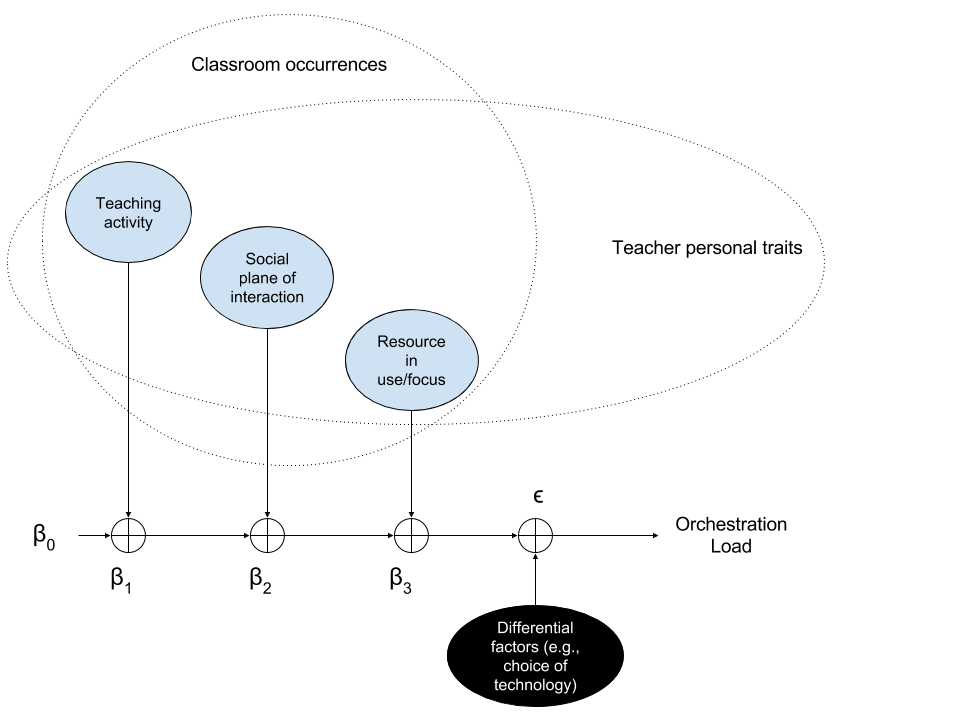
\includegraphics[width=\linewidth]{img/ModelFactorsOL}
\caption{A model of factors influencing orchestration load}
\label{fig:model}
\end{figure}

In the absence of prior knowledge about the relationship between these variables and orchestration load, we could propose a first approximation to the moment-to-moment orchestration load of a teacher as a linear combination of the variables:

\begin{multline}
\label{formOLScat}
OL = \beta_0 + \beta_A\times{}A + \beta_S\times{}S + \beta_F\times{}F \\ + \beta_E\times{}E + \beta_T\times{}T + \beta_H\times{}H + \epsilon
\end{multline}

In this formula, $A$ represents the current coordination activity (current coordination activity), $S$ is the current social plane of interaction, $F$ is the current resource in which the teacher is focusing, $E$ the teacher expertise, $T$ the familiarity of the teacher with the current technology or situation, and $H$ is the presence of an additional helper in the orchestration. To further operationalize the first three variables (what we called the `process variables'), we can transform each of them into a set of binary variables, each with its own $\beta$ coefficient: for episodes in which the teacher is, e.g., explaining a concept, the binary variable $A_{expl}$ would have a value of 1, while all the other variables about teacher activities (e.g., $A_{monit}$ for episodes in which the teacher is monitoring student work) would have a value of 0. 

%TODO: Maybe from here on could be removed, if we are short on space??
In the studies portrayed in section \ref{sec:eval}, we operationalized teacher coordination activities ($A$) in five mutually exclusive categories: explanation (i.e., lecturing), monitoring (student's work), questioning students, repairs (solving a student doubt), and task  distribution (including also transitions between tasks). Similarly, the social plane of teacher interactions was divided into class-wide, with small groups (of students), or with individual students. Also, the focus of the interaction was categorized into the main classroom elements, like the teacher's computer, the whiteboard, the classroom projector, students' own faces, etc. Thus, using this kind of representation, formula (\ref{formOLScat}) would be transformed into the following:

\begin{multline}
\label{formOLS}
OL = \beta_0 + \beta_{A1}\times{}A_{expl} + \beta_{A2}\times{}A_{monit} + ... \\ + \beta_{S1}\times{}S_{indiv} + ... + \beta_{F1}\times{}F_{stud} + ... + \\ + \beta_E\times{}E + \beta_T\times{}T + \beta_H\times{}H + \epsilon
\end{multline}

One interesting property of the model presented above is that the process variables (teaching activity, social plane of interaction, focus of the interaction) can be determined at any point in time by an observer with relative ease. On the other hand, the last line of factors like expertise, familiarity and external help, can be assumed to be constant during a classroom lesson, and can also be easily determined, or can even be manipulated by researchers (something we do in the validation studies of section \ref{sec:eval}). Hence, the only piece of information missing is a measure (or, at least, an estimation) of the total instantaneous orchestration load a teacher is facing at a certain moment of a lesson (OL, in formulas (\ref{formOLScat}) and (\ref{formOLS})).

% Pierre: in general, explain this better, longer!
%\begin{itemize}
%\item Classroom management/orchestration is assumed to be multi-tasking \cite{Doyle2006} in the sense of multiple constraints and concerns, but most often the orchestration is a \textit{sequence} of actions and decisions (put an example)
%\item From the definition of orchestration \cite{Dillenbourg2009}, we can see there are several \textit{process variables} that can affect the orchestration load at any point in time, but which may not be interesting for us when designing the technology: what is the current coordination \textit{activity} the teacher is performing, at which \textit{social plane} is the coordination happening, or what is the \textit{resource} (including objects and people) on which the activity is focusing
%\item The load that each process variable contributes may vary from teacher to teacher (personality, training...) and can be additionally modified/corrected due to other additional factors (teacher expertise, familiarity, external help...) (see Figure \ref{fig:model}). Hence, to have an idea of the load experienced by the teacher and enable meaningful comparison between two different classroom situations, we have to take into account the influence of such process variables (e.g., was there more explanation in one case than in the other? does this teacher experience more load while explaining than other activities?) (explain this more clearly and in detail!)
%\item Hence, as a first approximation to the instantaneous orchestration load, we could pose the following linear model:
%\item ...where A (current coordination activity) can be Explanation, Monitoring, Questioning etc. (i.e., for an individual teacher, different activities may represent different amounts of load); similarly, S (social plane) can be Individual, Small group, Class-wide; and F (focus of activity) can be the different classroom elements on which the teacher may focus, including students; etc. The process variables could be represented graphically as an orchestration graph, see \cite{prieto2011recurrent;dillenbourg2015orchestration}. 
%\item If we transform the categorical variables in Formula (\ref{formOLScat}) into binary variables, we are left with:
%\item In this model, as designers of technology, we are interested mostly on measuring the correction factor (weight?) on orchestration load due to our technologies (e.g., $\beta_T*T$), once we take away the effect of the known process variables (A, T, S), keeping the rest of the variables in the classroom situation as constant as possible.
%\item (clarify that the first line is observable, second line are the manipulable/manipulated variables ... we are only missing something to measure OL!)
%\end{itemize}



\section{Estimating Orchestration Load Using Physiological (Eye-tracking) and Behavioral Measures}
\label{sec:measures}
%TODO: Maybe this intro is too long, could be shortened if needed
As note above, we need a way of tracking the evolution of moment-to-moment orchestration load. This estimation of the total (instantaneous) orchestration load can be used, along with the other observed variables of our model (like the current teaching activity), to build statistical models that estimate the influence of each of these factors in the orchestration load. Once we have an idea of these influences (which, let us remember, may vary from teacher to teacher and from classroom to classroom), we can make meaningful comparisons between situations, and determine whether one represented distinctly more load than the other (and start disentangling why this is so).

In psychology and human factors research, cognitive load can be measured directly by performing a `dual task' experiment: analyzing the performance of individuals that do a secondary task (e.g., detecting a text in the screen changes color) while performing our primary task of interest (e.g., solving difficult arithmetic operations). This kind of method, however, poses problems when the activity of interest is already a complex multi-tasking one \cite{Paas2003} (like teaching is). Subjective measures of cognitive load (i.e., asking a person how much effort did a task take) are also possible, but have similar limitations to relatively short, atomic tasks, as they rely on the subject's memory of the event. Indeed, in our initial pilots in this line of research we had to discard repeated subjective measures of mental load throughout the lesson, as they disrupted too much the flow (and teachers' experience) of the lesson.

Once we rule out other direct measures of cognitive load like brain imaging (for obvious logistic reasons), this only leaves us with indirect measures of cognitive load \cite{Brunken2003}. Among these, physiological measures are the most popular ones (i.e., tracking involuntary reactions of the body to such increased load, like heart rate or pupillary dilation). Among these, mobile eye-tracking has the advantage of being applicable while performing everyday tasks like teaching, and it provides several measures that have been related to cognitive load in the literature \cite{boucsein2000engineering,Buettner2013}. In order to increase the reliability of our measurements, which are taken in uncontrolled conditions (as opposed to typical eye-tracking studies in the lab which carefully control lighting conditions, etc.), we can \textit{triangulate} across multiple such measures (e.g., use both pupillary diameter \textit{and} saccade speed).

The fact that mobile eye-trackers also provide a first-person audiovisual recording of the lesson from the point of view of the teacher also enables researchers to observe the process variables of our model (e.g., what the teacher is doing at a certain moment in the lesson), which can be manually coded by a human observer. Hence, we propose to use physiological data (from mobile eye-tracking technology), along with behavioral data (the manual coding of teachers' actions and social context from the first-person video feed), as a way to build moment-to-moment models of orchestration load such as those presented in section \ref{sec:model}. Our data analysis follows five main steps (see Figure \ref{fig:analysis}):

\begin{figure}[!t]
\centering
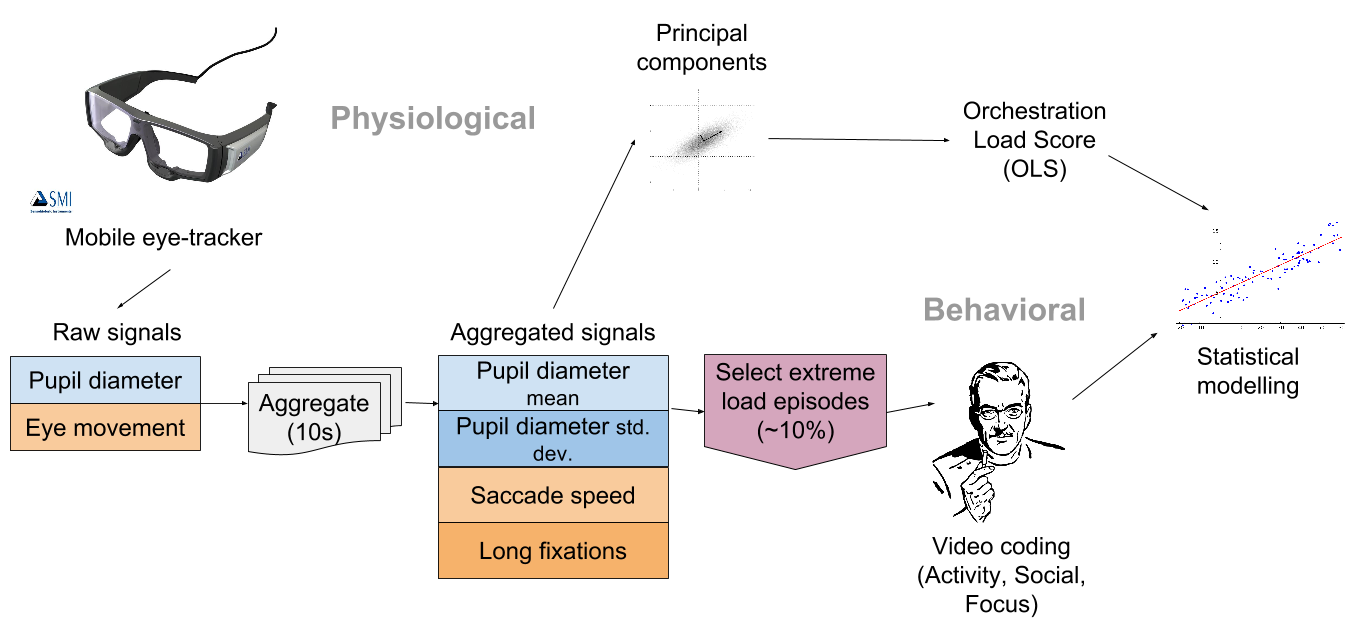
\includegraphics[width=\linewidth]{img/AnalysisMethodBase.png}
\caption{Diagram representing the physiological-behavioral analysis of orchestration load}
\label{fig:analysis}
\end{figure}

\begin{enumerate}
\item During the session, eye-tracking data and audiovisual feed of the lesson are recorded using a mobile eyetracker worn by the teacher (see Figure \ref{fig:case4picture}).
\item From the raw eye-tracking data, we take multiple measures that have been related to cognitive load\footnote{In our studies below, we have taken the four metrics that \cite{Buettner2013} found related to cognitive load, namely: pupil diameter mean, pupil diameter standard deviation, average saccade speed and number of fixations $>$500ms.}, we divide the lesson into windows or \textit{episodes} of a certain length\footnote{In the studies below, sliding windows of 10 seconds, with 5-second overlaps were chosen. This length was chosen striking a balance between them being short enough to capture variations in eye-tracking measures, and being long enough so that a human coder can easily discern the current behavioral variables (i.e., what the teacher is doing).}, and we aggregate those eye-tracking measures over each episode.
\item Since, at any point in time, the multiple eye-tracking metrics are not likely to correlate perfectly, we need a way to infer our estimation of instantaneous orchestration load ($OL$ in formula \ref{formOLS}) from these multiple values. In order to do that, a principal component analysis (PCA) is run over our whole dataset of load-related metrics for each episode, and the linear combination of measures that explains the most variance (i.e., the first component of the PCA) is chosen as our best estimation of the total instantaneous orchestration load (from now on, orchestration load score, or OLS)\footnote{Since PCA can provide two different solutions with opposite signs for each variable, the solution with most positive coefficients is chosen, as can be seen in Fig. \ref{fig:pca}. This solution not only is the most coherent with cognitive load literature (as all the selected measures are supposed to be directly correlated with load), it has also been validated against the ground truth of our case studies in section \ref{sec:eval}.}.
\item Each of the episodes comprising the lesson is manually coded in terms of the process variables of the model (current teaching activity, social plane of interaction and main focus of the teacher's gaze, see section \ref{sec:model})\footnote{Given that there can be several hundred such episodes in a 40-minute lesson, in the studies below we have done a purposeful \textit{sampling} of the episodes, taking only those in which \textit{all} four eyetracking metrics are either above or below the median of the session (what we could call ``agreement episodes''). This sampling tries to capture critical moments in terms of orchestration load \cite{Prieto2014}, and represents the episodes in which our four cognitive load-related metrics agree the load should be higher than average, or lower than average. In our experiments, using this sampling technique reduces the human effort to about 10\% of the episodes of a lesson.}.
\item We use machine learning techniques to build statistical models of the orchestration load of the lesson (e.g., in the form of a linear model, as proposed in section \ref{sec:model}). These models can be used to compare the load of two situations (see sections \ref{sec:study1}, \ref{sec:study2} and \ref{sec:study3} for examples of this kind of study), or just to extract insights about orchestration load of a classroom situation, in a non-comparative way (see section \ref{sec:study4} for an example of this kind of study).

\end{enumerate}

%\begin{itemize}
%\item At the most basic level, we want to track orchestration load (OL) in a moment-to-moment manner, in order to later take away the influence of process variables and find out if two situations had distinctly lower/higher load
%\item Since direct measurement of load (e.g., with dual-task) is problematic in complex multi-tasking activities \cite{Paas2003}, we have to resort to indirect measures (e.g., physiological)
%\item To estimate the influence of the process variables (teaching activity, social plane, focus of gaze) on load, we can resort to behavioral measures (i.e., observation of the classroom occurrences) -- e.g., through manual video coding
%\item Mobile eye-tracking can be used to obtain both relevant physiological data about cognitive load \cite{Buettner2013} and audiovisual feed for teacher behavior analysis without additional equipment (crucial when investigating in authentic settings). Indeed, we have shown the feasibility of this approach in explorations of orchestration load in the past \cite{Prieto2014,Prieto2015cscl,Prieto2015ectel}
%\item We propose the following method for analysis combining behavioral and physiological measures (see Figure \ref{fig:analysis}):
%\end{itemize}



\section{Case Studies}
\label{sec:eval}

\subsection{Methodology}

In order to provide initial evidence of the validity of the models and measures of orchestration outlined above, we have applied them in authentic classroom conditions, in several case studies spanning a total of 14 sessions. The sessions were orchestrated by four different teachers, with actual students at different educational levels (from 11-year-old learners to university students, see Table \ref{tab:cases}). The research questions that these case studies pursued could be summarized as follows:

\begin{description}
\item[RQ1] Are the aforementioned orchestration load score (OLS) and the proposed linear statistical models able to discriminate the load of substantially different classroom situations?
\item[RQ2] Can the application of these measures and models provide us with insights about the orchestration load of different classroom situations?
\end{description}

Among these four case studies, Study 1, 2 and 3 aimed at \textit{validating} the aforementioned model and physiological-behavioral measures (RQ1). In each of these validation studies we compared two orchestration situations which were similar in most aspects, but varied significantly in one of the additional factors mentioned in section \ref{sec:model} (namely, teacher expertise, familiarity with the classroom technology, and having additional help from a fellow orchestrator). In these studies, we make the assumption that one of the situations imposed a substantially higher orchestration load on the teacher than the other (e.g., having a helper would entail \textit{less} orchestration load than not having it). While it is debatable that the orchestration load was significantly higher \textit{at all moments} due to these factors, it is reasonable to suppose so for the aggregation of the whole session. Furthermore, this kind of ``weak experimental control'' is as much as we dared to manipulate otherwise realistic classroom situations, so as to maintain the authentic conditions that are the hallmark of orchestration-related research \cite{Roschelle2013}.

On the other hand, Study 4 was \textit{not} manipulated, and is rather provided as an illustrative example of how the models and methods can be used to extract insights about the orchestration load of a certain classroom situation (RQ2), in a unmanipulated, non-comparative manner.

Initial explorations of the datasets from Studies 1 and 4 have been published before \cite{Prieto2015cscl}, as is the case for part of the eyetracking data in Study 2 \cite{Prieto2015ectel}. However, the application of the statistical models and methods depicted in sections \ref{sec:model} and \ref{sec:measures} (the focus of this paper) is completely novel. Below, we describe the context and main results of the case studies. The anonymised datasets generated, full analytical code and detailed results are available online\footnote{\href{https://github.com/chili-epfl/paper-IEEETLT-orchestrationload}{https://github.com/chili-epfl/paper-IEEETLT-orchestrationload}.}.

In all four studies, we followed the data gathering and analysis methods described in section \ref{sec:measures}:

\begin{enumerate}
\item Eye-tracking data (including also subjective audiovisual feed) was recorded during lessons
\item Cognitive load-related metrics were calculated and aggregated for 10-second episodes
\item Principal Component Analysis was performed on the data from the four cases (see Figure \ref{fig:pca}) to obtain the orchestration load score (from the 1$^{st}$ principal component score of each episode)
\item We sampled "agreement episodes" the subjective audiovisual feed from the eye-tracker, and manually coded them by a single researcher, to extract the process variables of interest (teaching activity, social plane, and main focus of teacher's gaze)
\item Machine learning models were built using the OLS and video-coded variables (see each subsection below for descriptions of the concrete modelling)
\end{enumerate}


%\begin{itemize}
%\item The goals (research questions) of this paper are twofold:
%\begin{enumerate}
%\item Are the aforementioned PCA-based orchestration load score (OLS), and the proposed statistical models, able to discriminate the load of substantially different situations?
%\item Can the application of these measures and models provide us with insights about the orchestration load of different classroom situations?
%\end{enumerate}
%\item We have used the aforementioned approach and models for orchestration load in four case studies, spanning a total of 14 sessions orchestrated by four different teachers with actual students at different educational levels, from 11yrs old to university students (see Table \ref{tab:cases})
%\item The first three case studies aimed at validating the aforementioned model and physiological-behavioral measures (RQ1). In each of these validation studies we compared two orchestration situations which were similar in most aspects, but varied significantly in one aspect which we can assume is directly related to the teacher orchestration load (teacher expertise, familiarity with the classroom technology, having additional help from a fellow orchestrator). 
%\item While it is debatable that the situations had different inherent loads \textit{at all moments}, it is as much as we can manipulate and make comparations between inherently unique situations, while maintaining authenticity
%\item Finally, the fourth case study was not manipulated, and is provided as an illustrative example of how the models and methods can be used to extract insights about the orchestration load of a certain classroom/situation (RQ2)
%\item Initial explorations of the datasets from these cases have been published before for cases 1 and 4 \cite{Prieto2015cscl}, and for the first two sessions of case 2 \cite{Prieto2015ectel}. However, the application of the statistical models and methods depicted in sections \ref{sec:model} and \ref{sec:measures} is unpublished
%\item Below, we describe the context and main results of the case studies. The datasets generated, full analytical code and detailed results are available online\footnote{\href{https://github.com/chili-epfl/paper-IEEETLT-orchestrationload}{https://github.com/chili-epfl/paper-IEEETLT-orchestrationload}.}
%\item In all 4 studies the data gathering and analysis method of section \ref{sec:measures} was followed: a) eyetracking data was recorded and cognitive load-related metrics were aggregated for 10s episodes; b) Principal Component Analysis was performed on the data from the four cases (see Figure \ref{fig:pca}) to obtain the OLS (1st component score); c) "Extreme load episodes" were video coded by a single researcher, to extract the process variables (activity, social plane, focus of gaze) 
%\end{itemize}

\begin{figure}[!t]
\centering
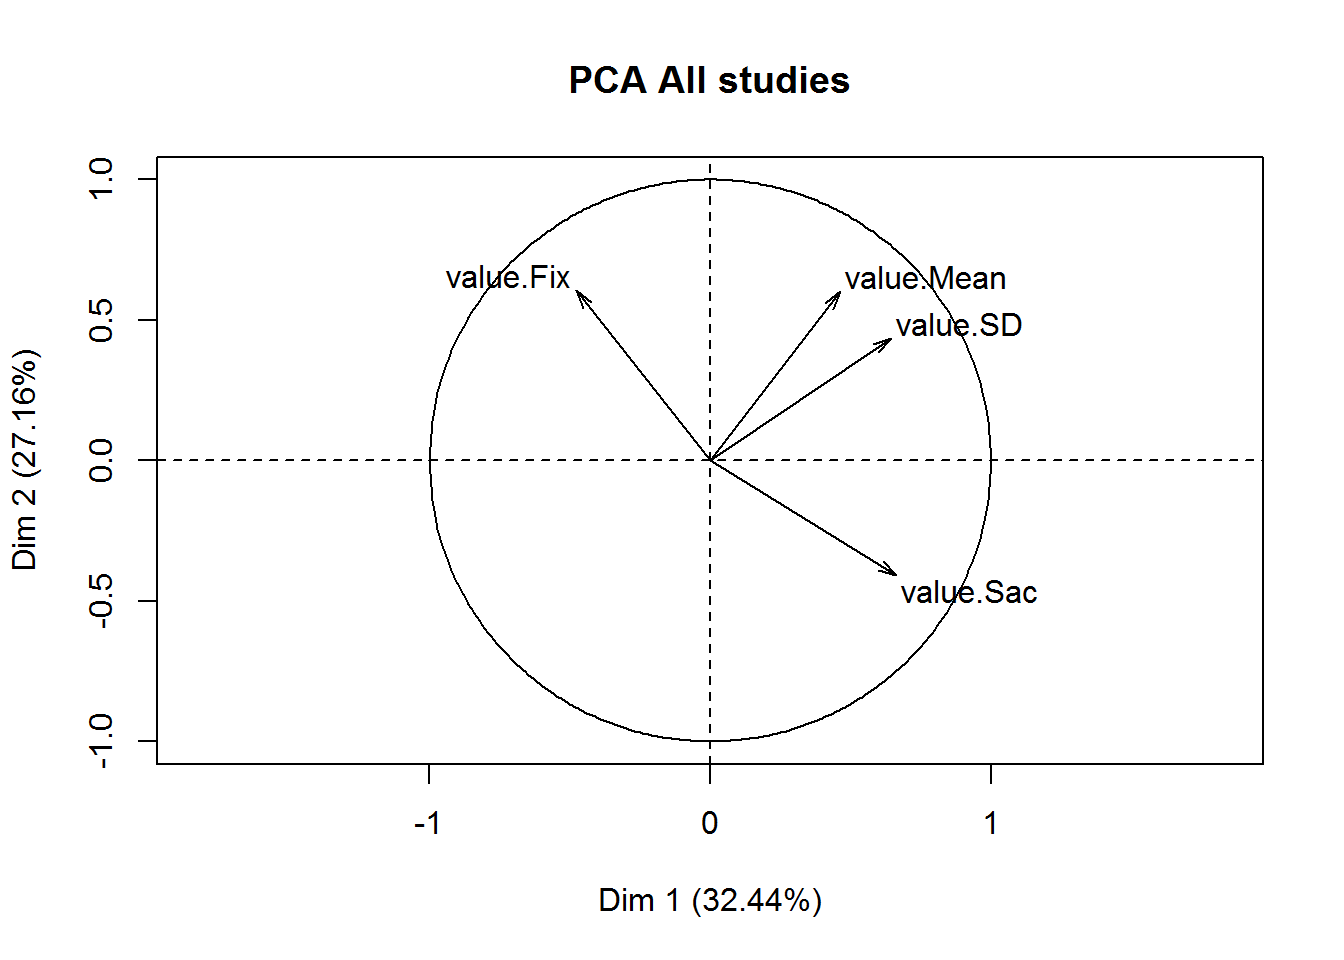
\includegraphics[width=\linewidth]{img/PCA.png}
\caption{Projection of the four eye-tracking measures recorded throughout the four case studies, on the space defined by the first two PCA components. The Orchestration Load Score (OLS) is the linear combination of the four measures, with loadings represented by the projection of the four measures on the \textit{horizontal} axis}
\label{fig:pca}
\end{figure}


\begin{table*}[!t]
%% increase table row spacing, adjust to taste
%\renewcommand{\arraystretch}{1.3}
% if using array.sty, it might be a good idea to tweak the value of
% \extrarowheight as needed to properly center the text within the cells
\caption{Summary of main case study characteristics}
\label{tab:cases}
\centering
%% Some packages, such as MDW tools, offer better commands for making tables
%% than the plain LaTeX2e tabular which is used here.
\begin{tabular}{|c||p{1.5cm}|p{1.5cm}|p{2cm}|p{3.4cm}|p{2cm}|p{3.4cm}|}
\hline
Study & Setting & Teachers & Sessions (session length) & Technological support & Main goal & Target variable\\
\hline
\hline
Case 1 & University & 1 expert, 1 novice & 2+1 (45-65' each) & Laptops, classroom projector & Validate measure/model & Teacher expertise (novice vs. expert) \\
\hline
Case 2 & Primary school & 1 expert & 2+2 (80' each) & Laptops, classroom projector vs. Tabletops, classroom projector & Validate measure/model & Familiarity with technology (usual vs. novel) \\
\hline
Case 3 & Open doors (primary) & 1 novice (researcher) & 4 (35-45' each) & Tabletops, classroom projector & Validate measure/model & External (human) help (without/with helper) \\
\hline
Case 4 & Open doors (primary) & 1 novice (researcher) & 3 (35-45' each) & Tabletops & Illustrate use & -- \\
\hline
\end{tabular}
\end{table*}



\subsection{Study 1: Exploring Teacher Expertise in an University Course}
\label{sec:study1}

One of the main factors that may affect orchestration load of a classroom situation is the amount of teacher experience, as more expert teachers have internalized and automatized many of the small tasks involved in classroom management \cite{feldon2007cognitive}, which have also been observed as ``routines'' in teachers of different levels of experience integrating new technologies in the classroom \cite{prieto2011recurrent}. Hence, more expert teachers will manage a classroom with more ease (i.e., with less orchestration load) than novice ones. In this first study, we explore the following particularization of RQ1 above: \textit{Is our modelling and OL score able to discriminate between similar learning situations, orchestrated by a novice and an experienced teacher?}.

%\begin{itemize}
%\item One of the factors that can affect orchestration load is teacher expertise (EXPERIENCE?): more expert teachers have internalized/automated many aspects of their teaching \cite{feldon2007cognitive,prieto2011recurrent} will manage the classroom with more ease (less load) than novice ones
%\item Case study question: \textit{Will our model and OL score be able to discriminate similar learning situations, orchestrated by a novel and an experienced teacher?}
%\end{itemize}

\subsubsection{Context}

The study took place during a real master-level course on ``Digital education and learning analytics'', held at EPFL (Switzerland). The lessons took place face-to-face, with students (10-12 of them, depending on the day) using their own laptops, and the teacher using laptop, projector and whiteboard (see Figure \ref{fig:case1picture}). The lesson plans combined fluidly lecturing, questioning of students and exercises. Two sessions were recorded for the experienced teacher (more than 10 years of teaching experience), and one for the novice teacher\footnote{Actually, two sessions were recorded for the novice teacher, but technical problems during the recording of one of them forced us to discard the data, as the situation would have been no longer similar to the ones recorded with the expert teacher.} (1 year of teaching experience). Session durations ranged from 45--65 minutes.


%\begin{itemize}
%\item Face-to-face master-level course on ``Digital education and learning analytics'' at EPFL. Classes had 10-12 students, working with laptops and teacher using laptop, projector and whiteboard (see Figure \ref{fig:case1picture}). The lessons were a fluid combination of lecture, questioning student and exercises
%\item Two lessons with the same student cohort were recorded for the expert teacher, and one for the novice teacher, 45-65min each (in reality, two sessions were recorded for each, but one of the novice sessions had to be thrown out due to technical problems during data gathering)
%\end{itemize}


\begin{figure}[!t]
\centering
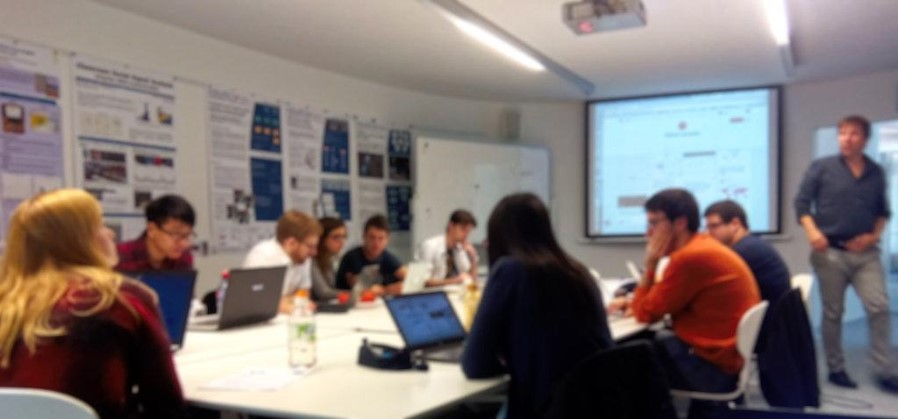
\includegraphics[width=\linewidth]{img/Case1Picture}
\caption{Classroom setup during Case study 1 (master-level course)}
\label{fig:case1picture}
\end{figure}

\subsubsection{Results}

To validate whether the model of factors and the proposed physiological measures (i.e., the orchestration load score -- OLS) represent a good predictor for orchestration load in this context, we assumed as a ``ground truth'' that the lessons orchestrated by the novice teacher represented a higher load (Load=1) than the ones orchestrated by the expert (Load=0). We trained a logistic regression model trying to predict this binary outcome (i.e., distinguish an episode orchestrated by the experienced teacher, vs. the novice one), using the three process variables coded by a human (teaching activity, social level of interaction, main focus of the gaze) and the OLS. 

As we can see in Table \ref{tab:case1results}, once we take away the influence of the process variables, the OLS still remains a significant predictor of the assumed (binary) orchestration load ($p<0.001$). Furthermore, this model including the OLS explains a considerable amount of the variance in the data (McFadden's pseudo-$R^2=0.88$). An analysis of variance of the different variables in the model confirms this, with the (eye-tracking-derived) OLS explaining most of the deviance in the data ($p<0.001$). %TODO: Check and put here what statistical test was done... ANOVA?

It is important to note that the two teachers in our study may differ in many other aspects affecting orchestration load, aside from the amount of teaching experience. Hence, this study provides only preliminary evidence that the proposed modelling (and the OLS as an approximation to moment-to-moment orchestration load) can distinguish high- vs. low-load situations in this kind of classroom context. In the following study, we test them in a context in which such personal differences are controlled.

%\begin{itemize}
%\item To validate whether the OLS is a good predictor for orchestration load in this context, we assume as a ground truth that the lessons orchestrated by the novice teacher represented a higher load (Load=1) than the ones orchestrated by the expert (Load=0). 
%\item We then train a logistic regression model to try to predict the aforementioned ``ground truth'' using the known process variables (activity, social, focus -- coded from the video by a researcher) and the OLS
%\item As we can see in table \ref{tab:case1results}, once we take away the influence of the process variables, the OLS still remains a significant predictor of the assumed (binary) orchestration load ($p<0.001$, see table \ref{tab:case1results}). Furthermore, this model including the OLS explains a considerable amount of the variance in the data (McFadden's pseudo-$R^2=0.88$) 
%\item An analysis of variance of the different variables in the model confirms this, with the OLS explaining most of the deviance in the data ($p<0.001$). 
%\item (Add disclaimer: of course, two teachers may differ in many ways, not only experience relates to load...)
%\end{itemize}

\begin{table}[!t]
%% increase table row spacing, adjust to taste
%\renewcommand{\arraystretch}{1.3}
% if using array.sty, it might be a good idea to tweak the value of
% \extrarowheight as needed to properly center the text within the cells
\caption{Logistic regression model to predict assumed orchestration load (1--Novice, 0--Expert teacher) in case study 1}
\label{tab:case1results}
\centering
%% Some packages, such as MDW tools, offer better commands for making tables
%% than the plain LaTeX2e tabular which is used here.
\begin{tabular}{|p{2.8cm}||r|r|r|r|}
\hline
Coefficient & Estimate & Std. error & z & p-value\\
\hline
\hline
Intercept (Monitoring, Class-level, Focus on student faces) & -2.65 & 1.51 & -1.75 & 0.08 \\
Activity: Explanation & -0.28 & 1.46 & -0.19 & 0.85 \\
Activity: Questioning & -1.93 & 1.90 & -1.02 & 0.31 \\
Activity: Repairs & 2.52 & 3.42 & 0.73 & 0.46 \\
Activity: Task distribution & -16.49 & 2765 & -0.01 & 1.00 \\
Social: Individual & 5.76 & 3.23 & 1.78 & 0.07 \\
Focus: Projector & -3.49 & 2.90 & -1.21 & 0.23 \\
Focus: Student computer & 1.00 & 1.72 & 0.58 & 0.56 \\
Focus: Table & 1.77 & 5.96 & 0.30 & 0.77 \\
Focus: Teacher computer & -2.04 & 1.40 & -1.45 & 0.15 \\
Focus: Whiteboard & -2.91 & 2.78 & -1.05 & 0.29 \\
\textbf{OLS} & \textbf{8.42} & \textbf{2.30} & \textbf{3.67} & \textbf{$<$0.001***} \\
\hline
\end{tabular}
\end{table}


\subsection{Study 2: Exploring Familiarity with Technology in a Primary School Classroom}
\label{sec:study2}

As mentioned in section \ref{sec:model}, another factor that is bound to affect the orchestration load experienced by a teacher in a lesson using technology, is the teacher's familiarity with the technology in use: a person trying out a tool for the first few times will not have yet developed automatisms to effortlessly use it in a classroom context, and hence will experience a higher orchestration load than during the usage of her usual set of tools. Hence, in this study we try to answer the question: \textit{Are our linear model and OLS able to discriminate learning situations orchestrated by a same teacher, using her usual and novel classroom technologies?}

%\begin{itemize}
%\item Another factor that can affect orchestration load in a predictable manner is familiarity with the technology: a teacher using a new tool will not have developed the necessary automatisms to effortlessly use it in the classroom \cite{feldon2007cognitive}, and hence will experience a higher orchestration load
%\item Case study question: \textit{Will our model and OL score be able to discriminate learning situations, orchestrated by a same teacher, but using her usual and novel classroom tools?}
%\end{itemize}

\subsubsection{Context}

In order to answer the aforementioned question, we conducted another study in the context of face-to-face lessons in an international Swiss secondary school. We recorded two sets of two math lessons, in which an experienced teacher (more than 20 years of teaching experience) taught to two different cohorts of students (18--22 students, aged 11--12) about geometry. In the first set of sessions, the teacher orchestrated students' work using a set of technologies she had used in previous courses (laptops with a geometry software\footnote{Geometer's Sketchpad, \href{http://www.dynamicgeometry.com/}{http://www.dynamicgeometry.com/}.}, a projector and a classroom management software\footnote{NetSupport School, \href{http://www.netsupportschool.com/}{http://www.netsupportschool.com/}}) with each of the cohorts. In the second set, the teacher orchestrated a collaborative groupwork game using a novel set of technologies (augmented paper tabletop interfaces based on Tinkerlamp \cite{do2012tinkerlamp}, and a projector as public display), with the same cohorts. Both classroom setups are portrayed in Figure \ref{fig:case2picture}.


%\begin{itemize}
%\item Face-to-face beginning of secondary school (11-12 yrs old), private international Swiss school, experienced teacher (more than 20 yrs experience), maths, two different cohorts of students (18-22 students each)
%\item Two sessions recorded while teacher orchestrated student work using laptops and a geometry software (Geometer's Sketchpad) as well as a classroom management software; two sessions recorded while teacher orchestrated student groupwork using a novel technology (augmented paper tabletop interfaces, based on Tinkerlamp \cite{do2012tinkerlamp} and public display/projector). See Figure \ref{fig:case2picture}
%\end{itemize}

\begin{figure*}[!t]
\centering
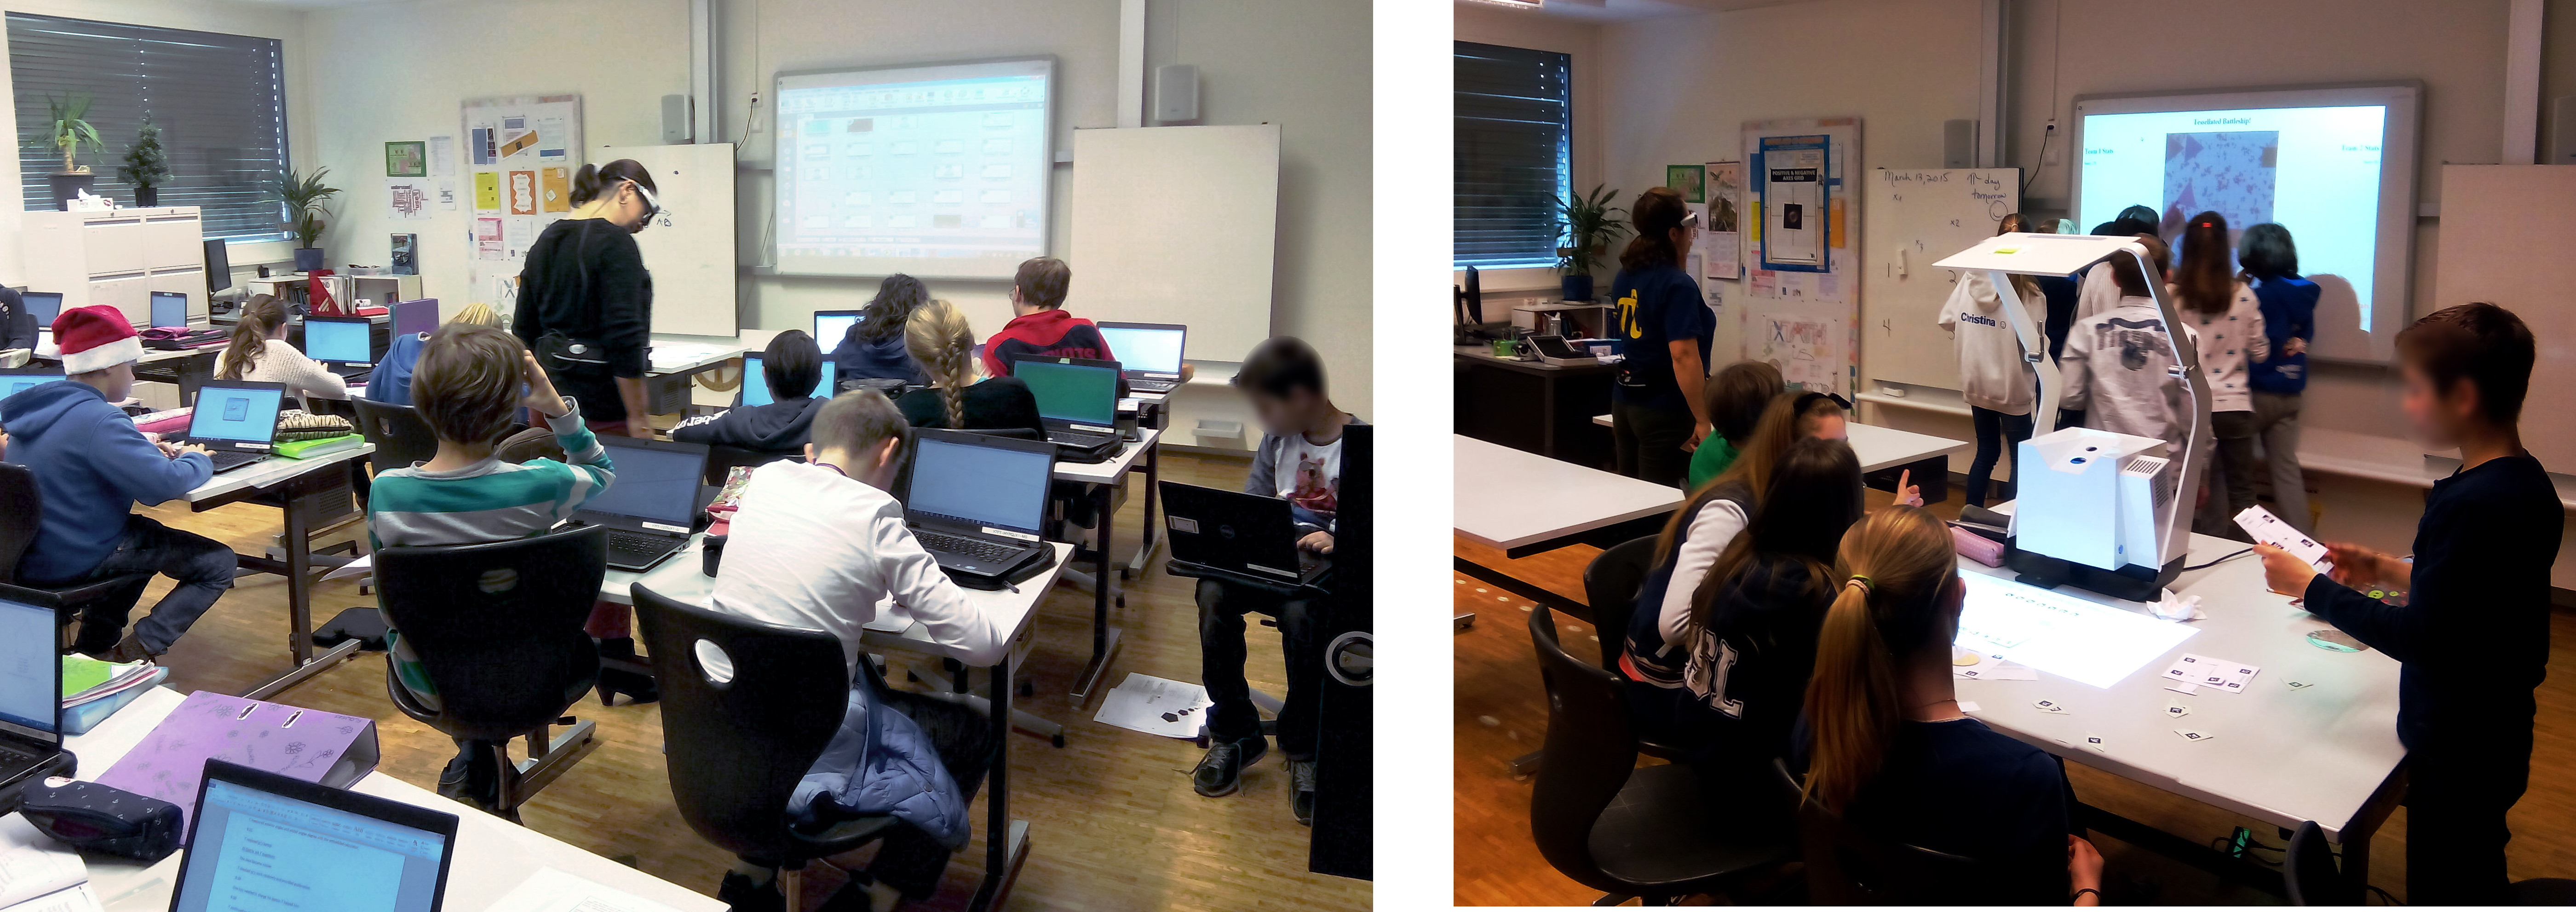
\includegraphics[width=\linewidth]{img/Case2Picture}
\caption{Classroom setup during two of the sessions in Case study 2: using usual laptop (left) and novel tabletop technology (right)}
\label{fig:case2picture}
\end{figure*}

\subsubsection{Results}

In a similar way as we did in the first study, to validate whether the OLS is a good predictor for orchestration load in this context, we assumed as the ground truth that the lessons orchestrated using novel technologies (for the teacher) represented a higher load (Load=1) than those using the usual classroom technology setup (Load=0). After extracting the OLS from the recorded eye-tracking metrics of every 10-second episode, and manually video-coding the teacher activity, social plane and focus of the gaze of the ``agreement episodes'' (as mentioned in section \ref{sec:measures}), we trained a logistic regression model to predict the ground truth from these variables.

As we can see in the coefficients of the logistic regression model (Table \ref{tab:case2results}), once we take away the influence of the process variables, the OLS still remains a significant predictor of the (binary) orchestration load ground truth ($p=0.002$). Furthermore, this model including the OLS explains a considerable amount of the variance in the data (McFadden's pseudo-$R^2=0.75$). An analysis of variance of the different variables in the model confirms this, with the OLS explaining an appreciable part of the deviance in the data ($p<0.001$). 

%TODO: This paragraph could be left out if we are in need of space
To interpret these results, we can assume that the personal characteristics of the teacher did not vary across conditions (since this was a within-subject study). Nevertheless, as usual in this kind of authentic setting studies, other factors (aside from familiarity with the technology) may have played a role in the respective orchestration load of both sets of sessions. Most important among these is the fact that lesson design (e.g., the teaching and learning activities performed) were not the same in both sets of sessions: the novel technology ones implied a less habitual way of managing the classroom (alternance between small-group collaboration and class-wide competition) than the usual technology ones (based on individual/pair linear work over a worksheet). However, this would only exaggerate the differences in orchestration load between usual and novel sessions, thus making the ground truth an ever more reasonable assumption. Therefore, this second study provides additional (albeit not definitive) evidence that the proposed model and measures of orchestration load might be applicable to a variety of authentic classroom settings.

%\begin{itemize}
%\item To validate whether the OLS is a good predictor for orchestration load in this context, we assume as a ground truth that the lessons orchestrated using novel technology represented a higher load (Load=1) than the ones orchestrated with the usual technology (Load=0). 
%\item We then train a logistic regression model to try to predict the aforementioned ``ground truth'' using the known process variables (activity, social, focus -- coded from the video by a researcher) and the OLS
%\item As we can see in table \ref{tab:case2results}, once we take away the influence of the process variables, the OLS still remains a significant predictor of the assumed (binary) orchestration load ($p=0.002$). Furthermore, this model including the OLS explains a considerable amount of the variance in the data (McFadden's pseudo-$R^2=0.75$) 
%\item An analysis of variance of the different variables in the model confirms this, with the OLS explaining an appreciable part of the deviance in the data ($p<0.001$). 
%\end{itemize}

\begin{table}[!t]
%% increase table row spacing, adjust to taste
%\renewcommand{\arraystretch}{1.3}
% if using array.sty, it might be a good idea to tweak the value of
% \extrarowheight as needed to properly center the text within the cells
\caption{Logistic regression model to predict assumed orchestration load (1--New classroom technology, 0--Usual technology) in case study 2}
\label{tab:case2results}
\centering
%% Some packages, such as MDW tools, offer better commands for making tables
%% than the plain LaTeX2e tabular which is used here.
\begin{tabular}{|p{2.8cm}||r|r|r|r|}
\hline
Coefficient & Estimate & Std. error & z & p-value\\
\hline
\hline
Intercept (Monitoring, Class-level, Focus on student faces) & 1.71 & 0.54 & 3.17 & 0.002** \\
Activity: Explanation & -2.91 & 0.71 & -4.08 & $<0.001$*** \\
Activity: Questioning & -4.46 & 0.91 & -4.88 & $<0.001$*** \\
Activity: Repairs & -2.55 & 0.91 & -2.81 & 0.005 \\
Activity: Task distribution & 0.31 & 0.87 & 0.36 & 0.72 \\
Social: Small group & 3.93 & 1.11 & 3.53 & $<0.001$*** \\
Social: Individual & -0.25 & 0.91 & -0.28 & 0.78 \\
Focus: Student laptop & -20.45 & 1577 & -0.01 & 0.99 \\
Focus: Paper elements & -2.31 & 0.74 & -3.14 & 0.002** \\
Focus: Projector & 20.92 & 2921 & 0.01 & 0.99 \\
Focus: Tabletop computer & 17.39 & 1758 & 0.01 & 0.99 \\
Focus: Teacher computer & -2.68 & 0.92 & -2.93 & 0.003** \\
\textbf{OLS} & \textbf{0.76} & \textbf{0.25} & \textbf{3.04} & \textbf{0.002**} \\
\hline
\end{tabular}
\end{table}


\subsection{Study 3: Exploring External Help in an Open Doors Day}
\label{sec:study3}

Following the (non-exhaustive) list of factors affecting orchestration load mentioned in section \ref{sec:model}, we can also conceive a third way of manipulating the orchestration load of a classroom situation. By providing the main teacher/orchestrator with an assistant, we postulate that her orchestration load during the lesson will be lowered\footnote{As long as clear, pre-defined roles and task distribution are performed beforehand among both facilitators, so that managing the assistant does not generate additional cognitive load.}. Hence, we performed a third study to validate the model and measures of orchestration load, looking at the following variant of our RQ1 question: \textit{Are our linear model and OLS measures able to discriminate between similar learning situations, orchestrated by a same teacher, but with/without an assistant orchestrator?}

%\begin{itemize}
%\item Finally, we can also manipulate orchestration load of a classroom situation by having the teacher have an assistant\footnote{With clear pre-defined roles and task distribution among both facilitators, so that managing the assistant does not generate additional load.}: we postulate that a teacher with an assistant will experience a lower orchestration load than one that has assistance
%\item Case study question: \textit{Will our model and OL score be able to discriminate similar learning situations, orchestrated by a same teacher, with and without an assistant orchestrator?}
%\end{itemize}

\subsubsection{Context}

To answer this question, we set up a semi-authentic study in the context of an open-doors day in our lab, in which cohorts of local school children (10--12 yrs old) from nearby public schools visit university labs. We transformed one of our rooms into a multi-tabletop classroom (Figure \ref{fig:case3picture}), and one member of the research team acted as the main facilitator of four math lessons, with different cohorts of visiting students (19--21 students each). The four sessions made use of augmented paper tabletops (based on Tinkerlamp \cite{do2012tinkerlamp}) and a public display/projector, and they alternated mini-lectures, small-group and whole-class exercises and games about geometry and coordinate systems. To manipulate the orchestration load, in two of the sessions the main orchestrator was aided by an assistant (but only in those moments where multiple groups were working independently, to ensure that the help was meaningful in terms of orchestration load -- something hard to achieve in moments of whole-class lecturing, for example). The groups of students that each orchestrator would monitor/help were decided beforehand, to avoid further coordination load during the session.

%\begin{itemize}
%\item Face-to-face math lessons enacted during an open-doors day in the lab with local school children (10-12 yrs old), public Swiss schools, novice teacher that was not the usual teacher (usual teachers present as passive observers), maths lesson combining mini-lecture, groupwork with tabletops and whole-class activity on projector (game), four different cohorts of students (19-21 students each)
%\item Four sessions recorded while teacher orchestrated the multi-tabletop classroom (augmented paper tabletop interfaces, based on Tinkerlamp \cite{do2012tinkerlamp} and public display/projector); in two of the sessions the assistant helped during the groupwork, dealing with half of the groups (in the rest of the lesson the assistant played no role). See Figure \ref{fig:case3picture}
%\item To answer the question about OLS as discriminator, only the relevant moments of the lesson (the groupwork) have been taken into account
%\end{itemize}

\begin{figure}[!t]
\centering
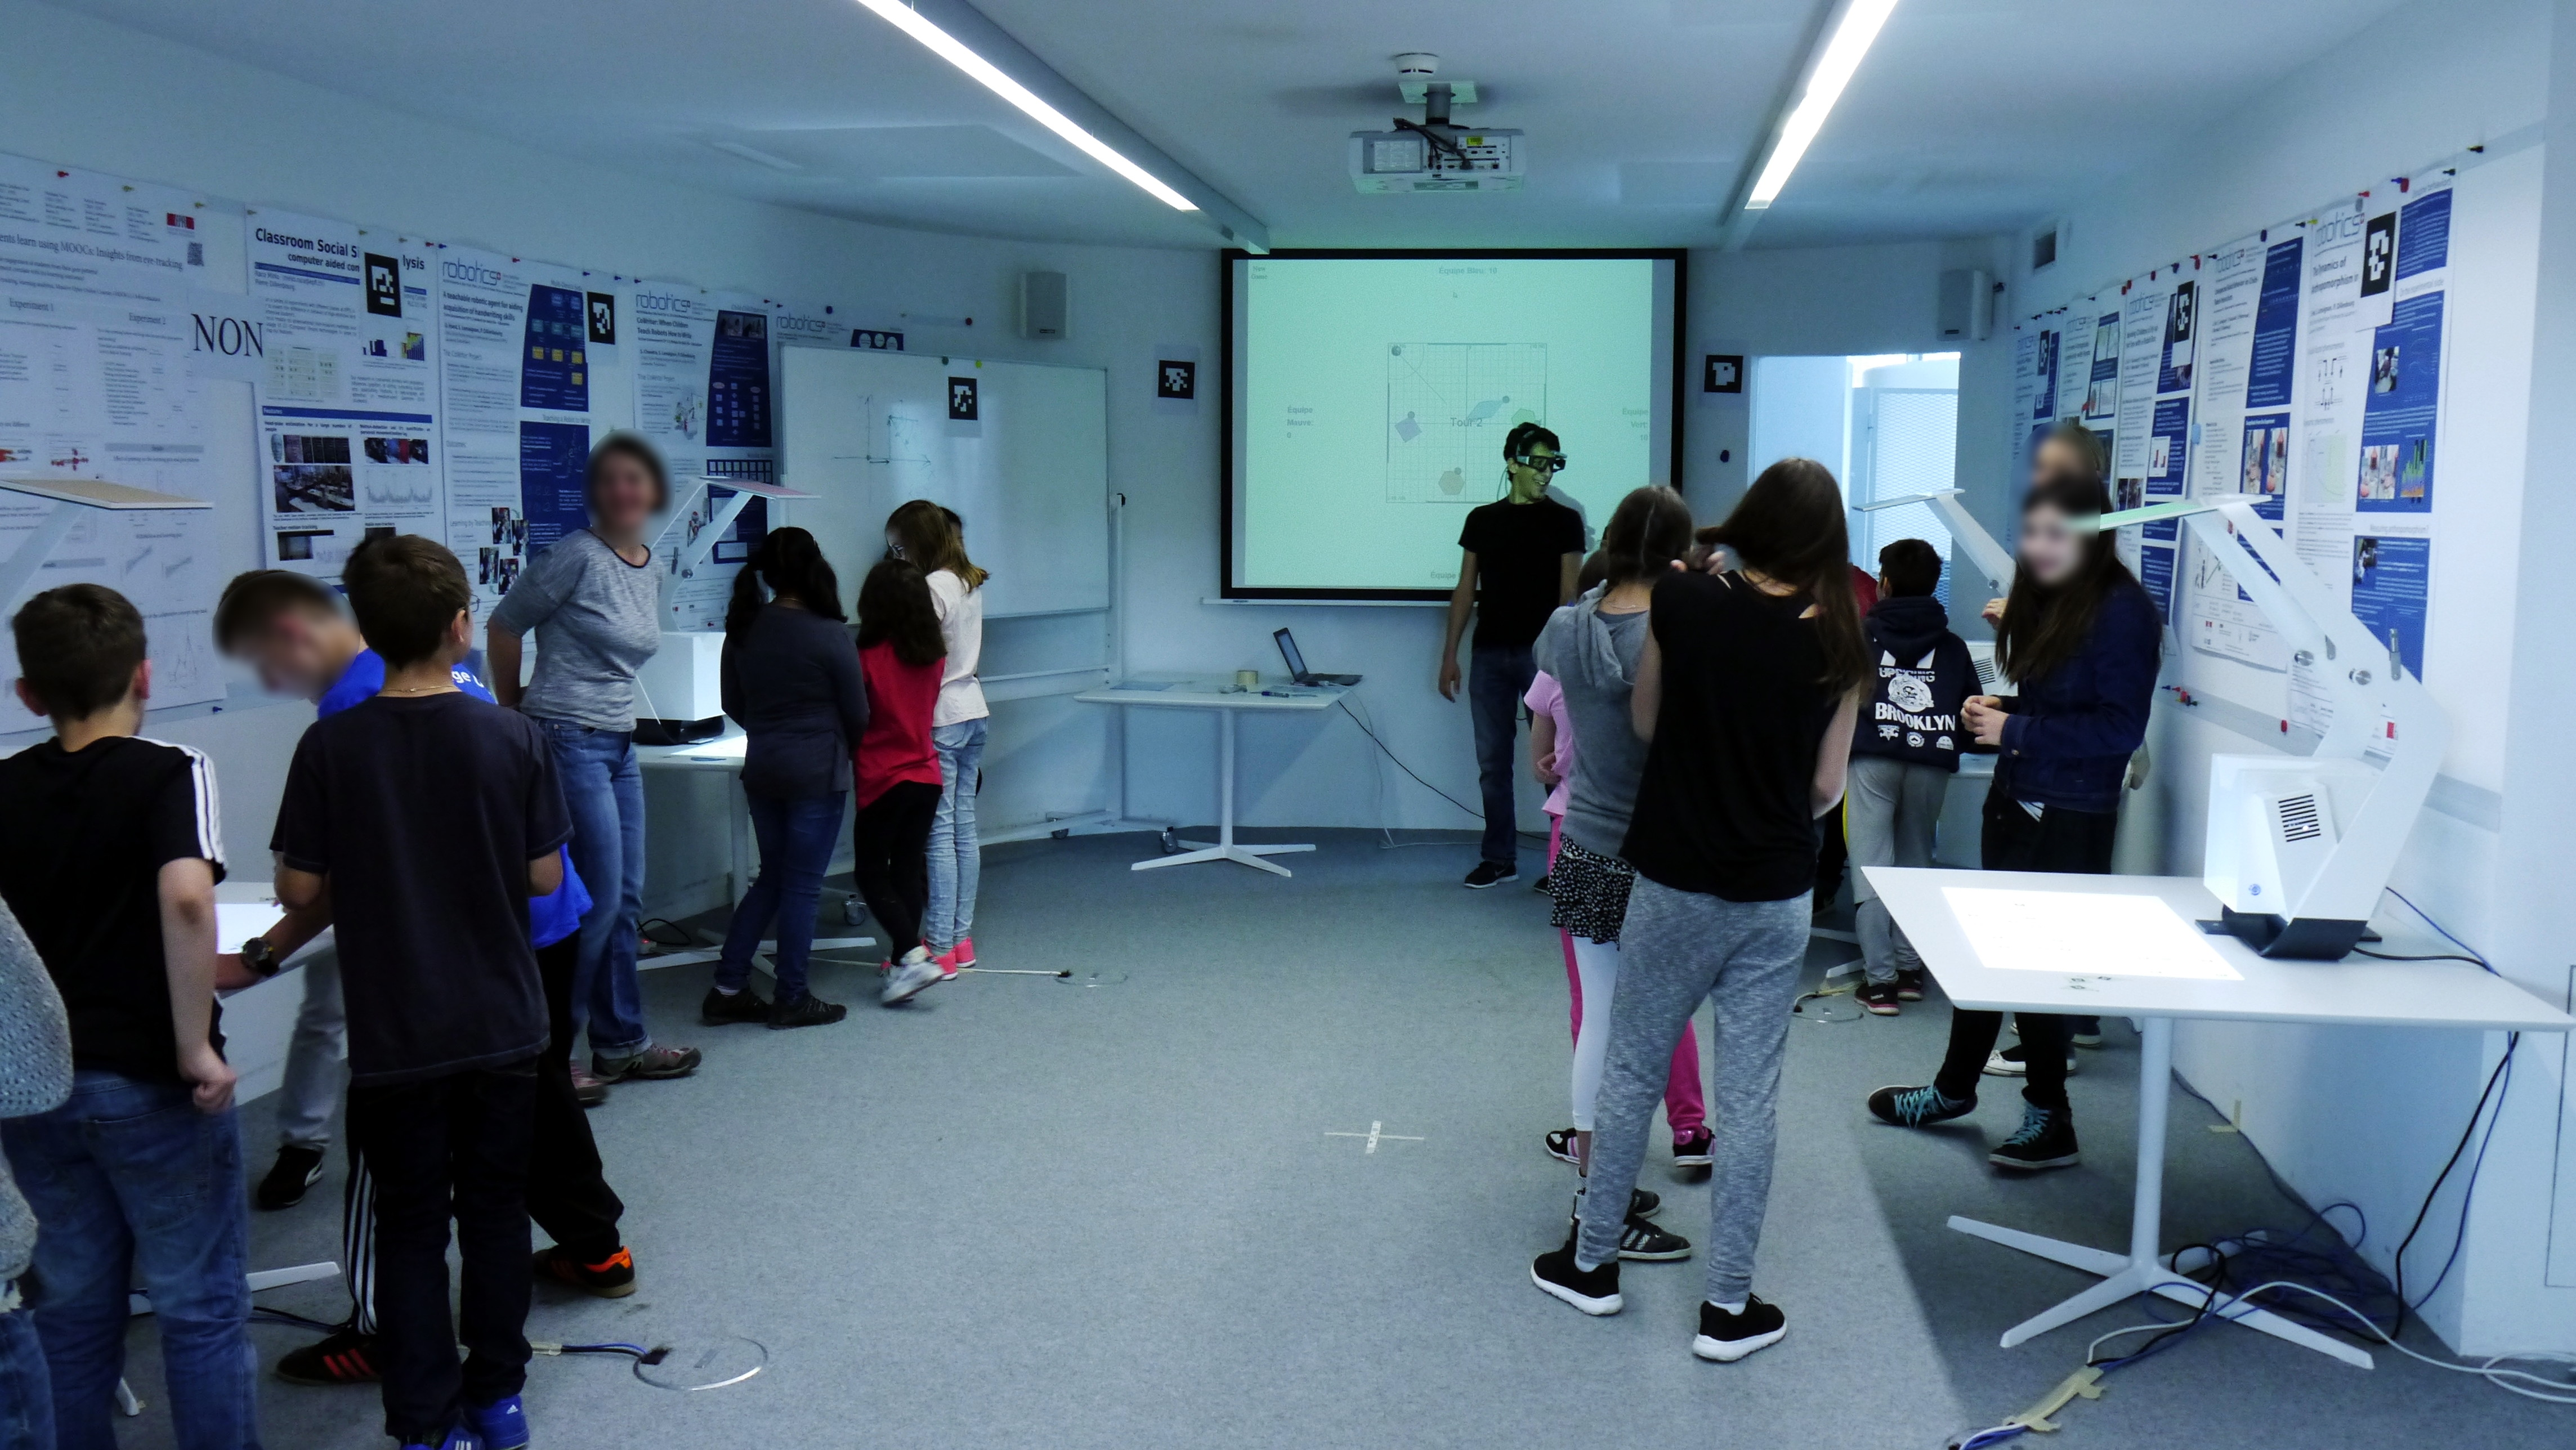
\includegraphics[width=\linewidth]{img/Case3Picture}
\caption{Classroom setup during Case study 3 (open-doors day)}
\label{fig:case3picture}
\end{figure}


\subsubsection{Results}

To validate whether the OLS is a good predictor for orchestration load in this study, taking into account our linear model of orchestration load, we assume as a ground truth that the lessons orchestrated without an assistant represented a higher load (Load=1) than the ones orchestrated with the assistant (Load=0). This is assumed to be true at least for the parts of the lesson where the assistant had a meaningful role. Hence, after following the same steps as in our previous studies (calculating OLS from eye-tracking measures, manual coding of agreement episodes), we selected \textit{only} the episodes falling in parts of the lesson plan where students were working independently (i.e., in which the assistant orchestrator, if present, had a meaningful role). Using these selected data, we trained a similar logistic regression model to predict the aforementioned ground truth using the known process variables (activity, social plane, focus -- from the video coding) and the OLS.

As we can see in Table \ref{tab:case3results}, once we take away the influence of the process variables, the OLS shows positive correlation (i.e., coefficient) with the ground truth. However, we found that in this model the OLS is no longer a \textit{significant} predictor of the binary orchestration load we assumed as ground truth ($p=0.13$). Furthermore, this model that includes the OLS explains relatively little variance in the data (McFadden's pseudo-$R^2=0.05$). One potential explanation for this lies in the fact that, by taking only a portion of the (rather short) lessons instead of multiple longer sessions, we are training our data in significantly less data (the model was trained on 163 agreement episodes, versus $~400$ episodes in each of the previous studies). Hence, the results of this study lead us to think that, either the load of monitoring half of the independently working student groups was not so high (as there were only 4 groups in total), or that we would have needed to record more sessions in order to detect such differences, when pinpointing this kind of sub-lesson timespan.

%\begin{itemize}
%\item To validate whether the OLS is a good predictor for orchestration load in this context, we assume as a ground truth that the lessons orchestrated without an assistant represented a higher load (Load=1) than the ones orchestrated with the assistant (Load=0) -- at least, for the parts of the lesson where the assistant had a role 
%\item To answer the question about OLS as discriminator, only the relevant moments of the lesson (the groupwork) have been taken into account
%\item We then train a logistic regression model to try to predict the aforementioned ``ground truth'' using the known process variables (activity, social, focus -- coded from the video by a researcher) and the OLS
%\item As we can see in table \ref{tab:case3results}, once we take away the influence of the process variables, the OLS shows clear, adequate trends (positive coefficient), but is no longer a significant predictor of the assumed (binary) orchestration load ($p=0.13$). Furthermore, this model including the OLS explains little variance in the data (McFadden's pseudo-$R^2=0.05$) 
%\item This may be due to the fact that we take only \textit{a portion} of the session, instead of whole sessions (the model is trained with 163 samples, versus $~400$ samples in the previous studies). We probably would have needed more data for OLS to detect the difference
%\end{itemize}

\begin{table}[!t]
%% increase table row spacing, adjust to taste
%\renewcommand{\arraystretch}{1.3}
% if using array.sty, it might be a good idea to tweak the value of
% \extrarowheight as needed to properly center the text within the cells
\caption{Logistic regression model to predict assumed orchestration load (1--Without assistant, 0--With assistant) in case study 3}
\label{tab:case3results}
\centering
%% Some packages, such as MDW tools, offer better commands for making tables
%% than the plain LaTeX2e tabular which is used here.
\begin{tabular}{|p{2.8cm}||r|r|r|r|}
\hline
Coefficient & Estimate & Std. error & z & p-value\\
\hline
\hline
Intercept (Monitoring, Class-level, Focus on student faces) & -0.09 & 0.62 & -0.15 & 0.88 \\
Activity: Questioning & 0.67 & 0.58 & 1.16 & 0.25 \\
Activity: Repairs & 0.95 & 0.41 & 2.30 & 0.02* \\
Activity: Task distribution & -0.37 & 0.64 & -0.58 & 0.56 \\
Social: Small group & -0.18 & 0.66 & -0.27 & 0.79 \\
Focus: Student backs & 1.65 & 1.27 & 1.30 & 0.19 \\
Focus: Projector & 0.11 & 0.71 & 0.15 & 0.88 \\
Focus: Tabletop computer & 0.88 & 0.72 & 1.23 & 0.22 \\
\textbf{OLS} & \textbf{0.86} & \textbf{0.57} & \textbf{1.51} & \textbf{0.13} \\
\hline
\end{tabular}
\end{table}


\subsection{Study 4: Modelling Orchestration Load in an Unmanipulated Setting}
\label{sec:study4}

Once we have initial validation that the OLS measure is a good tool to discriminate situations with different orchestration load (with the caveats found in study 3 about the amount of that used to build the statistical model), we can use it as a proxy measure of moment-to-moment orchestration load, in order to build models statistical models such as the one presented in section \ref{sec:model}. This will help us understand how the different process variables affect orchestration load in a certain classroom situation, and will enable us to extract patterns of higher or lower load, and compare different kinds of classroom situations. Below, we illustrate the usage of this measure in an unmanipulated setting, to answer a version of RQ2: \textit{What insights can we extract about the orchestration load in a multi-tabletop classroom, using a collaborative augmented paper game?}

%\begin{itemize}
%\item Once we have validated that the OLS is a good tool to discriminate situations with different orchestration load, we can use it as a measure of orchestration load, build models like that of Section \ref{sec:model} to understand how the different process variables affect load, extract patterns of higher or lower load, and compare different situations
%\item Below we illustrate how this measure can be used in an un-manipulated setting, an open doors day situation similar to that of case study 3
%\end{itemize}

\subsubsection{Context}

Similarly to the previous one, this study took place in a semi-authentic classroom situation in the context of another open-doors day in our lab, with three cohorts of students (aged 10--12) from local schools (14--25 students per cohort). Again, a member of the researcher team (a novice teacher) played the role of main orchestrator, with the usual teachers acting as passive observers (Figure \ref{fig:case4picture}). The three recorded sessions had an identical lesson plan, in which the orchestrator combined mini-lectures with collaborative exercises around augmented paper tabletops \cite{caballero2014single}. In this kind of classroom context, we wanted to undestand which were the main orchestration load trends and patterns (i.e., what kind of episodes represented higher or lower loads).

%\begin{itemize}
%\item Face-to-face math (SIMULATED) lessons enacted during an open-doors day in the lab with local school children (10-12 yrs old), public Swiss schools, novice teacher that was not the usual teacher (usual teachers present as passive observers), maths lesson about fractions combining mini-lecture and groupwork game with augmented paper tabletops, three different cohorts of students (14-25 students each)
%\item Three sessions recorded while teacher orchestrated the multi-tabletop classroom (augmented paper tabletop interfaces, based on Tinkerlamp \cite{do2012tinkerlamp} and public display/projector). See Figure \ref{fig:case4picture}
%\end{itemize}

\begin{figure}[!t]
\centering
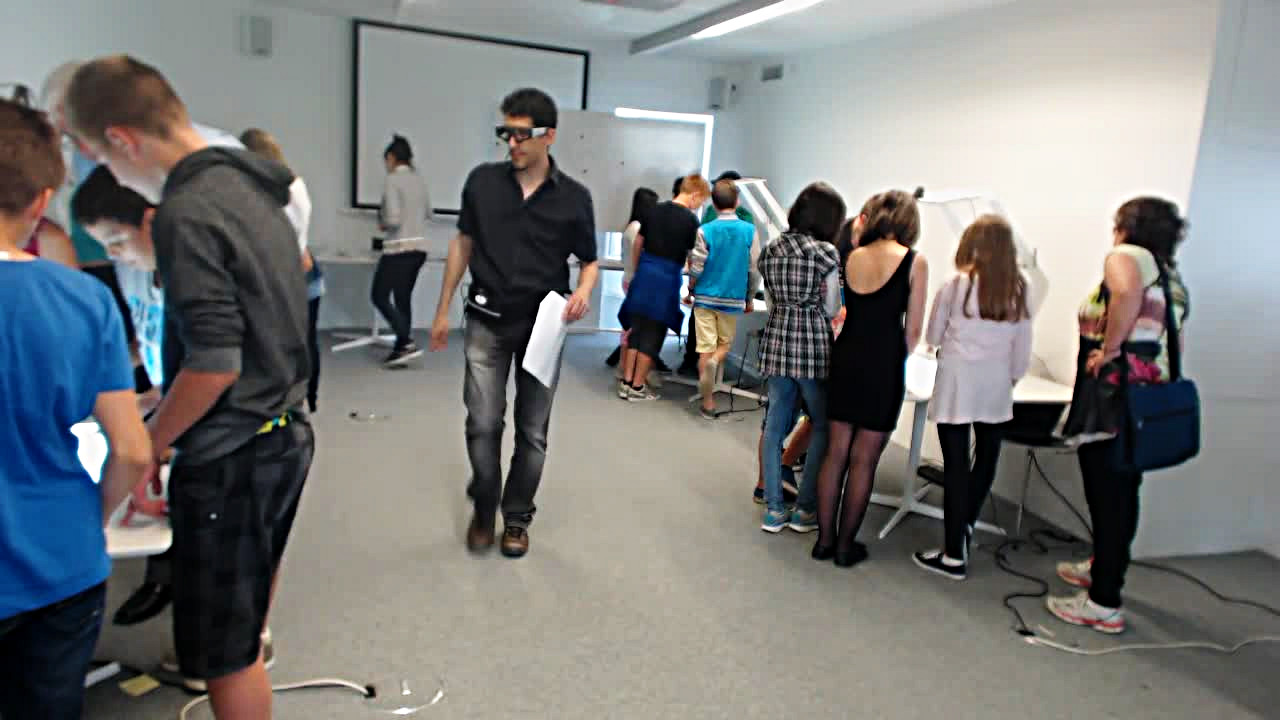
\includegraphics[width=\linewidth]{img/Case4Picture}
\caption{Classroom setup during Case study 4 (unmanipulated open-doors day)}
\label{fig:case4picture}
\end{figure}

\subsubsection{Results}

To get these orchestration load trends, after calculating the OLS and video-coding the agreement episodes, we trained a linear regression model to try to predict OLS using the known process variables observed from the subjective video (teaching activity, social plane, focus of the gaze), plus the session (i.e., we also wanted to know if one session had been noticeably more load than the others). The resulting model explains approximately 50\% of the variance in OLS, and an analysis of the variance of the model shows that the social plane of interaction, the focus of the gaze and the session were all significant predictors ($F=157$ with $p<0.001$; $F=46$ with $p<0.001$; and $F=22$ with $p<0.001$, respectively), while the teaching activity was only marginally significant ($F=2.59$ with $p=0.05$).

As we can see in Table \ref{tab:case4results}, the main significant trends (i.e., those coefficients that are significant predictors) are: a) that small-group interactions tended to be lower load than the reference level (class-level interactions); b) that looking at students' backs was lower load than looking at their faces (the reference level); or c) that looking at the tabletop itself tended to be lower load. Finally, we also see that d) the second and third sessions were on average higher load than the first session.

We can also speculate about the reasons behind these trends, not directly from the model, but from our contextual knowledge of the classroom situation (or observation of the videos). Class-level interactions may represent higher load than small-group ones due to the teacher needing to track and model the understanding of more students simultaneously (aside from keeping in mind the content of the lesson); the fact that student backs have no meaningful information to read about the progress of the students (as opposed to their faces, which may have) can be linked to the second trend. The other two trends initially seem counter-intuitive: however, the fact that the orchestrator was one of the designers of the tabletop application, and hence knew really well the user interface, might have lead to lower loads when looking at the tabletop; the expectation that session 1 would be more load than the others (due to the novelty of the situation) might have been offset by the fact that the three sessions occurred almost back-to-back (and hence the fatigue might have had a greater role than the relative novelty of the first session). However, this kind of post-hoc rationalizations of the evidence should be taken rather cautiously, as usual in many studies on the physiological measuring of cognitive load.

%\begin{itemize}
%\item To get the main orchestration load trends and patterns, we train a linear regression model to try to predict OLS using the known process variables (activity, social, focus -- coded from the video by a researcher), plus (e.g., if we want to know which session was more difficult)
%\item As we can see in table \ref{tab:case4results}, the linear model built with the process variables and the session predicts approximately 50\% of the variance in OLS
%\item An analysis of variance of the linear model shows that the social plane of interaction, the focus of the gaze and the session number were significant predictors in this model of OLS ($F=157; p-value<0.001$, $F=46; p-value<0.001$ and $F=22; p-value<0.001$), while the teaching activity itself was not ($F=2.59; p-value=0.05$)
%\item As we can see in Table \ref{tab:case4results}, the main significant trends are that the small-group of interaction was lower load than the reference (class-level) one; that looking at student backs was lower load than looking at their faces; so was looking at the tabletop itself; and that sessions 2 and 3 were higher load than session 1
%\item The reasons behind these trends cannot be directly deduced from the model, and need contextual or qualitative analysis of the video to develop conjectures: backs have no info to read the situation (EXPLAIN), while faces do; the facilitator was the designer of the tabletop app, so the UI was easy to read for him; maybe tiredness in sessions 2 and 3?
%\end{itemize}

\begin{table}[!t]
%% increase table row spacing, adjust to taste
%\renewcommand{\arraystretch}{1.3}
% if using array.sty, it might be a good idea to tweak the value of
% \extrarowheight as needed to properly center the text within the cells
\caption{Linear regression model to predict the orchstration load score (OLS) in case study 4}
\label{tab:case4results}
\centering
%% Some packages, such as MDW tools, offer better commands for making tables
%% than the plain LaTeX2e tabular which is used here.
\begin{tabular}{|p{2.6cm}||r|r|r|r|}
\hline
Coefficient & Estimate & Std. error & t & p-value\\
\hline
\hline
Intercept (Monitoring, Class-level, Focus on student faces, Session 1) & -0.02 & 0.11 & -0.22 & 0.82\\
Activity: Explanation & 0.01 & 0.07 & 0.14 & 0.89\\
Activity: Repairs & -0.001 & 0.05 & -0.02 & 0.98\\
Activity: Task distribution & -0.05 & 0.07 & -0.80 & 0.43\\
\textbf{Social: Small group} & \textbf{-0.29} & 0.12 & -2.44 & \textbf{0.02*}\\
\textbf{Focus: Student backs} & \textbf{-0.38} & 0.13 & -2.90 & \textbf{0.004**}\\
Focus: Teacher desk & 0.06 & 0.14 & 0.43 & 0.67\\
\textbf{Focus: Tabletop computer} & \textbf{-0.90} & 0.11 & -8.43 & \textbf{$<$0.001***}\\
\textbf{Session: 2} & \textbf{0.30} & 0.05 & 5.79 & \textbf{$<$0.001***}\\
\textbf{Session: 3} & \textbf{0.29} & 0.05 & 5.53 & \textbf{$<$0.001***}\\
\hline
\end{tabular}
\end{table}


\section{Discussion}
\label{sec:discussion}

\subsection{Eye-tracking Measures to Estimate Orchestration Load}

Regarding our first research question (are we able to discriminate the load of substantially different classroom situations?), the results from studies 1, 2 and 3 support the notion that the Orchestration Load Score (OLS), obtained from multiple eye-tracking metrics as described in section \ref{sec:measures}, provides a discriminant measure of teachers' orchestration load, obtainable in authentic classroom settings. These results (especially those of case 3) also show some of the limitations of the proposed method: for instance, the fact that a certain amount of data (i.e., number of 10-second episodes) is needed to discriminate the orchestration load of different classroom situations (i.e., taking only small parts of a session might not lead to clearly distinguishable OLS scores).

Although we cannot claim that this OLS is generalizable to any classroom situation, the fact that our studies were set in a variety of classroom settings using different classroom technologies, gives us hope about the wideness of its applicability. Nevertheless, further comparative studies in authentic settings, with ``reasonable ground truths'' (such as those described in sections \ref{sec:study1}--\ref{sec:study3}) should be performed to continue the validation of these methods.

Another important limitation of the methods for modelling and measuring orchestration load presented here, is the fact that these methods are quite expensive (both in terms of equipment and human effort, since they require researcher manual work to code the process variables from the eyetracking videos). However, as eye-tracking technology becomes cheaper (together with the fact that the measures used do not require high accuracy in terms of gaze pointing), this problem may go away. Furthermore, the behavioral video coding can also be made cheaper through crowdsourcing (since the process variable categories chosen are relatively simple to assess, even for non-researchers), or even automation (applying machine learning techniques on eye-tracking and other wearable sensor data \cite{prieto2016teaching}).

Besides these limitations, several open issues and questions remain about the usage of these models and measures of orchestration load. For example, one may ask how invasive these methods are and how ``authentic'' is a classroom situation in which the teacher wears a quite conspicuous pair of goggles and an additional researcher observer is present. Leaving aside the fact that mobile eye-tracking technology is becoming more discrete (with recent prototypes barely distinguishable from normal glasses), in our studies all teachers stated that after a few minutes they forgot about wearing the googles; most students, similarly, never seemed to notice or comment on the goggles beyond the first five minutes of the lesson.

It should also be noted that the list of process variables in our orchestration load model (teaching activity, social plane of interaction, focus of the gaze/interaction) is not an exhaustive one: one could also look at the effect of each individual student, the effect of disciplinary remarks, or many other variables affecting class management. Similarly, the coding scheme chosen here for each of those variables is not exempt from improvement: for instance, a research effort focused on inquiry-based learning might want to categorize teaching activities in a more pedagogy-specific manner, to understand how different activities in the support of inquiries may affect orchestration load.

Finally, we should also note that alternative models of orchestration load are also possible: one could argue that, given the complex nature and business of teaching, ``the load of the teacher is always 100\%'', and what actually varies is the capacity and stress levels (and hence, the performance) of the orchestrator: some teachers may handle an individual model of the understanding of each student, while less capable ones may bunch all students' understanding into a single variable. Further research is needed to understand which of these models reflects more accurately different classroom situations.


%\begin{itemize}
%\item The results from case studies 1, 2, 3 support the notion that OLS, obtained through the method presented in Section \ref{sec:measures}, provides a discriminant measure of teachers' cognitive load, obtainable in authentic classroom settings
%\item These results (sp. case 3) also show some of the limitations of the method -- a certain volume of data is needed for OLS to discriminate the load of different situations (e.g., several sessions, not just small parts of sessions)
%\item The OLS measure cannot be said to be generalizable yet to any classroom situation, but it has worked in a variety of settings -- and more semi-controlled comparative studies in a variety of settings with more teachers should be performed to continue validating it
%\item The method is still quite expensive in terms of equipment and effort, and requires quite a bit of researcher manual work... but this is changing as ETs become cheaper (not much accuracy needed). The behavioral coding of process variables can also be made cheaper with crowdsourcing (categories are quite simple to assess even for non-experts), and there is initial evidence that machine learning methods could automate this process \cite{prieto2016teaching}
%\item Open Qs: Are the situations really authentic (observers, ETs)? subjects did not complain and kids were not distracted after the initial minutes. Furthermore, eyetracker technology is becoming more discrete
%\item Open Qs: These process variables are not exhaustive, and the codes are not the last word -- further research can find other variables, and other ways of coding them that are more meaningful (generic or pedagogy-specific)
%\item Open Qs: Alternative models of OL: maybe CL is always 100\%, and maybe some people can handle more stuff than others with that load -- maybe find ways of factoring in the performance, subjective sensation of stress...
%\end{itemize}

\subsection{Orchestration Load Patterns and Learning Technology Insights}

Our second research question inquired about the insights that could be derived from these kinds of studies about the orchestration load of different classroom situations. Study 4 above illustrates how the OLS and the manually-coded process variables can be used to build statistical models of orchestration load and to extract initial insights about the orchestration load trends and patterns of a classroom situation. By applying the same kind of methods to the data of all the studies presented so far, we can get insights about the kind of influence that these different variables have on orchestration load, at different levels of specificity. Table \ref{tab:trends} summarizes the main orchestration load trends of each study, and of different aggregations within our dataset\footnote{For the sake of clarity and brevity, Table \ref{tab:trends} shows only the effect sizes using Cohen's $d$ (the difference in the means standardized by the variability of the data) of those predictors that are significant at the 0.05 level. For a more complete analysis, please head to the paper's accompanying analytical code and dataset at  \href{https://github.com/chili-epfl/paper-IEEETLT-orchestrationload}{https://github.com/chili-epfl/paper-IEEETLT-orchestrationload}.}.

At the single-study level, we can see for instance how in study 1 the episodes in the reference level (teacher monitoring at the whole-class level, looking at student faces) is the only significant predictor, although we can notice how the average OLS for these episodes was higher for the novice than for the expert teacher (which responds to our expectations). In case study 2, the same teacher had significantly higher loads while explaining or questioning to students when using the novel tabletop technology, even if looking at the tabletops themselves was appreciably less load than the reference level (monitoring the class while looking at faces).

Joining the data from multiple case studies (2\textsuperscript{nd} and 3\textsuperscript{rd} columns from the right in Table \ref{tab:trends}) we can, for instance, make comparisons between the orchestration load patterns of laptop classrooms versus those of multi-tabletop classrooms (with the obvious caveats given the very small sample sizes, as we only have data from 2-3 different teachers in each setting). We can see how, in the tabletop classrooms both the reference level (monitoring at the class-level, looking at students), questioning episodes and tabletop-related technical problem-solving tend to be \textit{high} load (a trend not so apparent in the more traditional laptop classrooms). In the laptop classrooms, we can see how task distribution episodes, and the focus on the whiteboard, seem to be \textit{lower} load. We can also see several common orchestration load trends across both kinds of classroom technology setups (see next).

Joining the data from all the studies presented here (1\textsuperscript{st} column from the right in Table \ref{tab:trends}), we can start extracting some general trends (with the aforementioned caveats regarding sample size) about how the different process variables seem to affect orchestration load. In this model, most of the variables seem to be significant predictors of orchestration load: the reference-level episodes (monitoring, class-level, looking at student faces) tend to be higher load, while the teacher focusing on tabletops, her own leptop, or the whiteboard, tend to be lower load. Regarding the social plane of interaction, both small-group and individual interactions seem to be noticeable lower load than class-level ones.

From the learning technology designer's point of view, these insights and trends rais an interesting issue. According to these measures and models, the influence of technology on orchestration load \textit{does not seem to be a direct one} (i.e., larger loads are not necessarily tied to looking at the technology user interfaces), but rather an indirect one, as the choice of technology modifies the mix of teaching activities and social planes (and the manner and time spent on each of them). This may imply that, at the classroom level, different classroom technologies (and probably also novel pedagogical designs that are tied with them) vary the orchestration load by \textit{changing what teachers do}, and how difficult this new mix of activities is. For instance, the introduction of a new technology may increase the uncertainty of the learning situation, provoking that more effort is put into trying to read student faces (not in looking more intently at the technology \textit{per se}). This kind of indirect relationship between orchestration load and classroom technology, in turn, supports the idea of studying orchestration in realistic classroom conditions, as opposed to a lab setting (where focus is often forced on direct technology usage and measuring load/performance of such direct use). At the same time, these insights seem to support several of the existing guidelines for the ``design of orchestrable technology'' in the literature, such as providing support for teacher awareness of the learning process \cite{dillenbourg2013design} (e.g., powered by learning analytics). In any case, we should not forget that these results and implications are extracted from a limited dataset of classroom studies, and therefore are not guaranteed to be generalizable to every teacher and classroom setting. However, as more studies of this kind are performed, more generalizable and trustworthy insights will undoubtedly emerge.

%\begin{itemize}
%\item Case study 4 illustrates how the OLS, behavioral variables and statistical models can be used to extract insights about the orchestration load of a classroom situation
%\item Applying the same kind of modelling to the data of all our studies, we can begin to get insights into the kind of influence that these process variables have on orchestration load (Table \ref{tab:trends}, the complete data analysis and results is available online\footnote{\href{https://github.com/chili-epfl/paper-IEEETLT-orchestrationload}{https://github.com/chili-epfl/paper-IEEETLT-orchestrationload}.}) 
%\item For example, in case study 1, the reference episodes (monitoring, class-level, looking at student faces), was appreciably lower load for the expert teacher (while for the novice it was higher)
%\item In case study 2, the same teacher had significantly higher loads while explaining or questioning to students when using the novel tabletop technology, even if looking at the tabletops themselves was appreciably less load than monitoring the class while looking at faces
%\item Joining the data from multiple case studies, we can make comparisons between laptop classrooms vs. tabletop ones: the reference monitoring at the class-level is higher load in the tabletop classroom,  questioning episodes or tabletop-related technical problems were higher load too, in the tabletops there were more moments of looking at student backs (even if they are lower load). Also commonalities in both kinds of classrooms: individual and group-level interaction was lower load, looking at the teacher computer was lower load
%\item Furthermore, joining the data from all the cases, we also can start extracting some general trends in how the different process variables seem to affect orchestration load: the reference (monitoring, class-level, faces) are higher load, other social levels and focuses were lower load than faces, technical problems were even higher load than monitoring
%\item Additional aspects are noteworthy: the influence of technology on load \textit{does not seem to be direct} (when looking at the UI), but rather it modifies the mix of teaching activities. \textit{Different classroom technologies} (and probably also new pedagogical designs) \textit{change what teachers do, and how difficult each teaching activity is} -- e.g., by increasing the uncertainty of the situation, so more effort is put into reading student faces
%\item This supports the idea of studying orchestration in realistic classroom conditions, not just in the lab (where focus is often forced on measuring direct technology usage). Also, it seems to support some of the existing "design for orchestration" guidelines, such as providing (learning analytics-powered) support for teacher awareness of the learning process \cite{dillenbourg2013design}.
%\item But, again, these results are extracted from a very limited dataset and are not guaranteed to be generalizable. More studies needed!
%\end{itemize}

\begin{table*}[!t]
%% increase table row spacing, adjust to taste
%\renewcommand{\arraystretch}{1.3}
% if using array.sty, it might be a good idea to tweak the value of
% \extrarowheight as needed to properly center the text within the cells
\caption{Summary of the statistically-significant process variable factors and their effect sizes (in terms of Cohen's $d$ \cite{cohen1977statistical})}
\label{tab:trends}
\centering
%% Some packages, such as MDW tools, offer better commands for making tables
%% than the plain LaTeX2e tabular which is used here.
\begin{tabular}{|p{3cm}||p{1.2cm}|p{1.2cm}|p{1.2cm}|p{1.2cm}|p{1.2cm}|p{1.2cm}|p{1.2cm}|p{1.2cm}|p{1.2cm}|}
  \hline
Case & 1       & 1       & 2       & 2       & 3       & 4       & 1+2     & 2+3+4   & 1+2+3+4 \\ 
  \hline
  Teacher & A       & B       & C       & C       & D       & D       & A+B+C   & C+D     & A+B+C+D \\ 
  \hline
  Expertise & Expert & Novice & Expert & Expert & Novice & Novice & Varied & Varied & Varied \\ 
  \hline
  Technology & Laptops + Projector   & Laptops + Projector   & Laptops + Projector   & Tabletops + Projector & Tabletops + Projector & Tabletops only      & Laptops + Projector   & Tabletops           & Varied              \\ 
  \hline
  Students & Young adults & Young adults & 11-12yrs     & 11-12yrs     & 10-12yrs     & 10-12yrs     & Varied       & 10-12yrs     & Varied       \\ 
  \hline
  No.sessions &  2 &  1 &  2 &  2 &  4 &  3 &  5 &  9 & 14 \\ 
  \hline
  No.episodes &  142 &   49 &  236 &  166 &  667 &  332 &  427 & 1165 & 1592 \\ 
  \hline
  Adjusted $R^2$ of model & 0.11 & 0.30 & 0.39 & 0.29 & 0.48 & 0.44 & 0.16 & 0.45 & 0.35 \\ 
  \hline
   \hline
  Reference (Monitoring, Class-level, Focus on student faces) & -0.72 &  +1.15 &     &     &  +0.70 &     &     &  +0.66 &  +0.45 \\ 
   \hline
  Activity: Explanation (lecturing) &   &   &   & +1.1 &   &   &   &   &   \\ 
   \hline
  Activity: Solve technical problems &    &    &    &    &    &    &    & +0.47 & +0.48 \\ 
   \hline
  Activity: Questioning &    &    &    & +0.97 &    &    &    & +0.30 &    \\ 
   \hline
  Activity: Task distribution &    &    &    &    &    &    & -0.5 &    &    \\ 
   \hline
  Social: Small-group &     &     &     &     & -0.70 &     &     & -0.63 & -0.51 \\ 
   \hline
  Social: Individual &     &     & -0.77 &     &     &     & -0.50 & -0.78 & -0.69 \\ 
   \hline
  Focus: Student backs &     &     &     &     & -0.51 & -0.68 &     & -0.68 & -0.50 \\ 
   \hline
  Focus: Table or desk &     &     &     &     &     &     &     &     & -0.77 \\ 
   \hline
  Focus: Pieces of paper &     &     & -0.51 & -0.98 &     &     & -0.55 & -0.58 & -0.63 \\ 
   \hline
  Focus: Projector &     &     &     & -1.13 & -0.49 &     &     & -0.54 & -0.41 \\ 
   \hline
  Focus: Student laptops &    &    &    &    &    &    &    &    & -0.3 \\ 
   \hline
  Focus: Tabletop computers &     &     &     & -1.09 & -0.92 & -1.80 &     & -1.07 & -0.98 \\ 
   \hline
  Focus: Teacher's computer &     &     & -0.88 &     & -0.40 &     & -0.51 & -0.32 & -0.61 \\ 
   \hline
  Focus: Whiteboard &     &     &     &     &     &     & -0.61 &     & -0.65 \\ 
   \hline
\end{tabular}
\end{table*}


\section{Conclusion}
\label{sec:conclusion}

In this paper we presented an overview of what orchestration load is, and a method to quantify it by combining physiological and behavioral measures (i.e., eye-tracking metrics and manual video coding of the orchestration episodes). The results of applying these methods to four studies encompassing 14 sessions orchestrated by four different teachers in a variety of settings, support the Orchestration Load Score (a linear combination of four eye-tracking metrics related to cognitive load) as a discriminant measure of orchestration load. Our studies show how this measure, along with orchestration process variables like teaching activity or social plane of interaction, can distinguish between situations in which it is reasonable to presume different levels of cognitive load (teachers with different levels of experience, novel vs. usual classroom technologies, and --only partially-- having a human assistant). By building statistical models of orchestration load (which assume OLS as a reliable measure of orchestration load), we also obtained first glimpses into disentangling the respective influence of different factors on orchestration load (e.g., using different classroom technology setups).

These promising results, however, are not without limitations, mostly related to the small sample sizes in terms of number of teachers and classroom technologies tested (which are related to the high costs and risks involved in this kind of classroom experiments). Hence, future work along this line of research should be directed towards further validation studies of these methods at a larger scale and in different classroom settings (something that can be aided by sharing anonymized datasets and analytical code/methods, as we do in this paper\footnote{See \href{https://github.com/chili-epfl/paper-IEEETLT-orchestrationload}{https://github.com/chili-epfl/paper-IEEETLT-orchestrationload}.}). Other interesting paths for future research involve the reuse and modification of the methods presented here, for instance by using further process variables, different statistical models and video coding schemes, or using (and triangulating) different physiological measures related to workload (e.g., heart rate for cognitive load, accelerometers to track physical load, etc.).

Once these methods have been validated more thoroughly in a variety of classroom settings, and wearable sensor technologies have become more affordable, the methods presented here can be added along to our toolbox of usability methods as classroom technology designers. These methods can be applied as well to more general educational research (e.g., understanding the orchestration load of different pedagogical methods, using what we called elsewhere ``multimodal teaching analytics'' \cite{prieto2016teaching}). Indeed, the methods presented here could also be applicable beyond the realm of education, in many other human activities that are highly social and involve heavy multi-tasking (e.g., healthcare, knowledge workers, etc.) -- what we could call ``multimodal professional analytics''.

%\begin{itemize}
%\item This paper presented the notion of orchestration load, a model to try to quantify it, and a method to measure it using with mobile eyetrackers complemented with behavioral analysis (video coding)
%\item Our results in 4 case studies, 14 sessions, 4 teachers support OLS (a linear combination of 4 ET measures related to cognitive load) as a discriminant measure of orchestration load (comparing teacher expertise, novel/usual technology and --partially-- having an assistant)
%\item The statistical models built accepting OLS as a reliable measure of load, provide a first glimpse of how different kinds of classroom episodes influence the load of teachers in different kinds of technological setups
%\item Problem: Still very costly?? setting up access to classrooms, sensors, risk of discard data, manual coding... maybe mention in passing
%\item Future work: different process variables and coding schemes, different non-linear models of orchestration load, other sensors of load (accelerometers for physical load, e.g., skin conductance? heart rate? EEG?)
%\item Need to share datasets (but with privacy) so that we can get reliable methods, measures and models for classroom usability that can be used in real settings (and maybe at scale!)
%\item Could even be extended to study other professions and activities that are complex, social, ... in their natural setting
%\end{itemize}




% if have a single appendix:
%\appendix[Proof of the Zonklar Equations]
% or
%\appendix  % for no appendix heading
% do not use \section anymore after \appendix, only \section*
% is possibly needed

% use appendices with more than one appendix
% then use \section to start each appendix
% you must declare a \section before using any
% \subsection or using \label (\appendices by itself
% starts a section numbered zero.)
%




% use section* for acknowledgment
\ifCLASSOPTIONcompsoc
  % The Computer Society usually uses the plural form
  \section*{Acknowledgments}
\else
  % regular IEEE prefers the singular form
  \section*{Acknowledgment}
\fi

This research was supported by a Marie Curie Fellowship within the 7\textsuperscript{th} European Community Framework Programme (MIOCTI, FP7-PEOPLE-2012-IEF project no. 327384). Special thanks also go to Patrick Jermann, the International School of Lausanne and all the student and teacher participants in EPFL's ``Journ\'ee des classes'' open-doors events.

%\begin{itemize}
%\item The authors would like to thank... Marie Curie, students and teachers participating in JdC's
%\item Should we acknowledge ISL school, Patrick explicitly? or keep them anonymous?
%\end{itemize}


% Can use something like this to put references on a page
% by themselves when using endfloat and the captionsoff option.
\ifCLASSOPTIONcaptionsoff
  \newpage
\fi



% trigger a \newpage just before the given reference
% number - used to balance the columns on the last page
% adjust value as needed - may need to be readjusted if
% the document is modified later
%\IEEEtriggeratref{8}
% The "triggered" command can be changed if desired:
%\IEEEtriggercmd{\enlargethispage{-5in}}

% references section

% can use a bibliography generated by BibTeX as a .bbl file
% BibTeX documentation can be easily obtained at:
% http://mirror.ctan.org/biblio/bibtex/contrib/doc/
% The IEEEtran BibTeX style support page is at:
% http://www.michaelshell.org/tex/ieeetran/bibtex/
\bibliographystyle{IEEEtran}
% argument is your BibTeX string definitions and bibliography database(s)
\bibliography{orchload}
%
% <OR> manually copy in the resultant .bbl file
% set second argument of \begin to the number of references
% (used to reserve space for the reference number labels box)
%\begin{thebibliography}{1}
%\bibitem{IEEEhowto:kopka}
%H.~Kopka and P.~W. Daly, \emph{A Guide to \LaTeX}, 3rd~ed.\hskip 1em plus
%  0.5em minus 0.4em\relax Harlow, England: Addison-Wesley, 1999.
%
%\end{thebibliography}

% biography section
% 
% If you have an EPS/PDF photo (graphicx package needed) extra braces are
% needed around the contents of the optional argument to biography to prevent
% the LaTeX parser from getting confused when it sees the complicated
% \graphics command within an optional argument. (You could create
% your own custom macro containing the \includegraphics command to make things
% simpler here.)
%\begin{IEEEbiography}[{\includegraphics[width=1in,height=1.25in,clip,keepaspectratio]{mshell}}]{Michael Shell}
% or if you just want to reserve a space for a photo:

%\begin{IEEEbiography}[{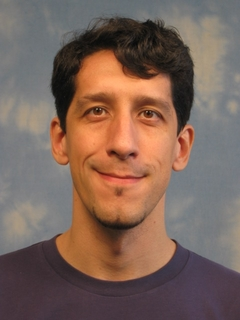
\includegraphics[width=1in,height=1.25in,clip,keepaspectratio]{img/LPPhoto.jpg}}]{Luis P. Prieto} received his Ph.D. in Information and Communication Technologies from the University of Valladolid. He is a Marie Curie Fellow at the CHILI Lab in the \'Ecole Polytechnique F\'ed\'erale de Lausanne (EPFL). His research interests include classroom orchestration, distributed and augmented paper learning technologies, and the use of wearable technologies to capture and understand complex practice with ICT and use it for reflection. He has authored more than fifty academic publications on these topics, and he is a member of IEEE and ACM.
%\end{IEEEbiography}
%
%
%\begin{IEEEbiography}[{
\includegraphics[width=1in,height=1.25in,clip,keepaspectratio]{img/Sharma.png}}]{Kshitij Sharma}
% is ...
%\end{IEEEbiography}
%
%\begin{IEEEbiography}[{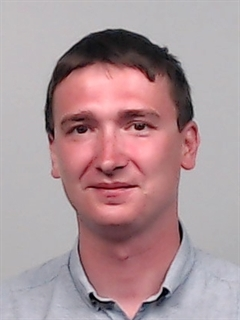
\includegraphics[width=1in,height=1.25in,clip,keepaspectratio]{img/Kidzinski.jpg}}]{{\L}ukasz Kidzinski}
% is ...
%\end{IEEEbiography}
%
%\begin{IEEEbiography}[{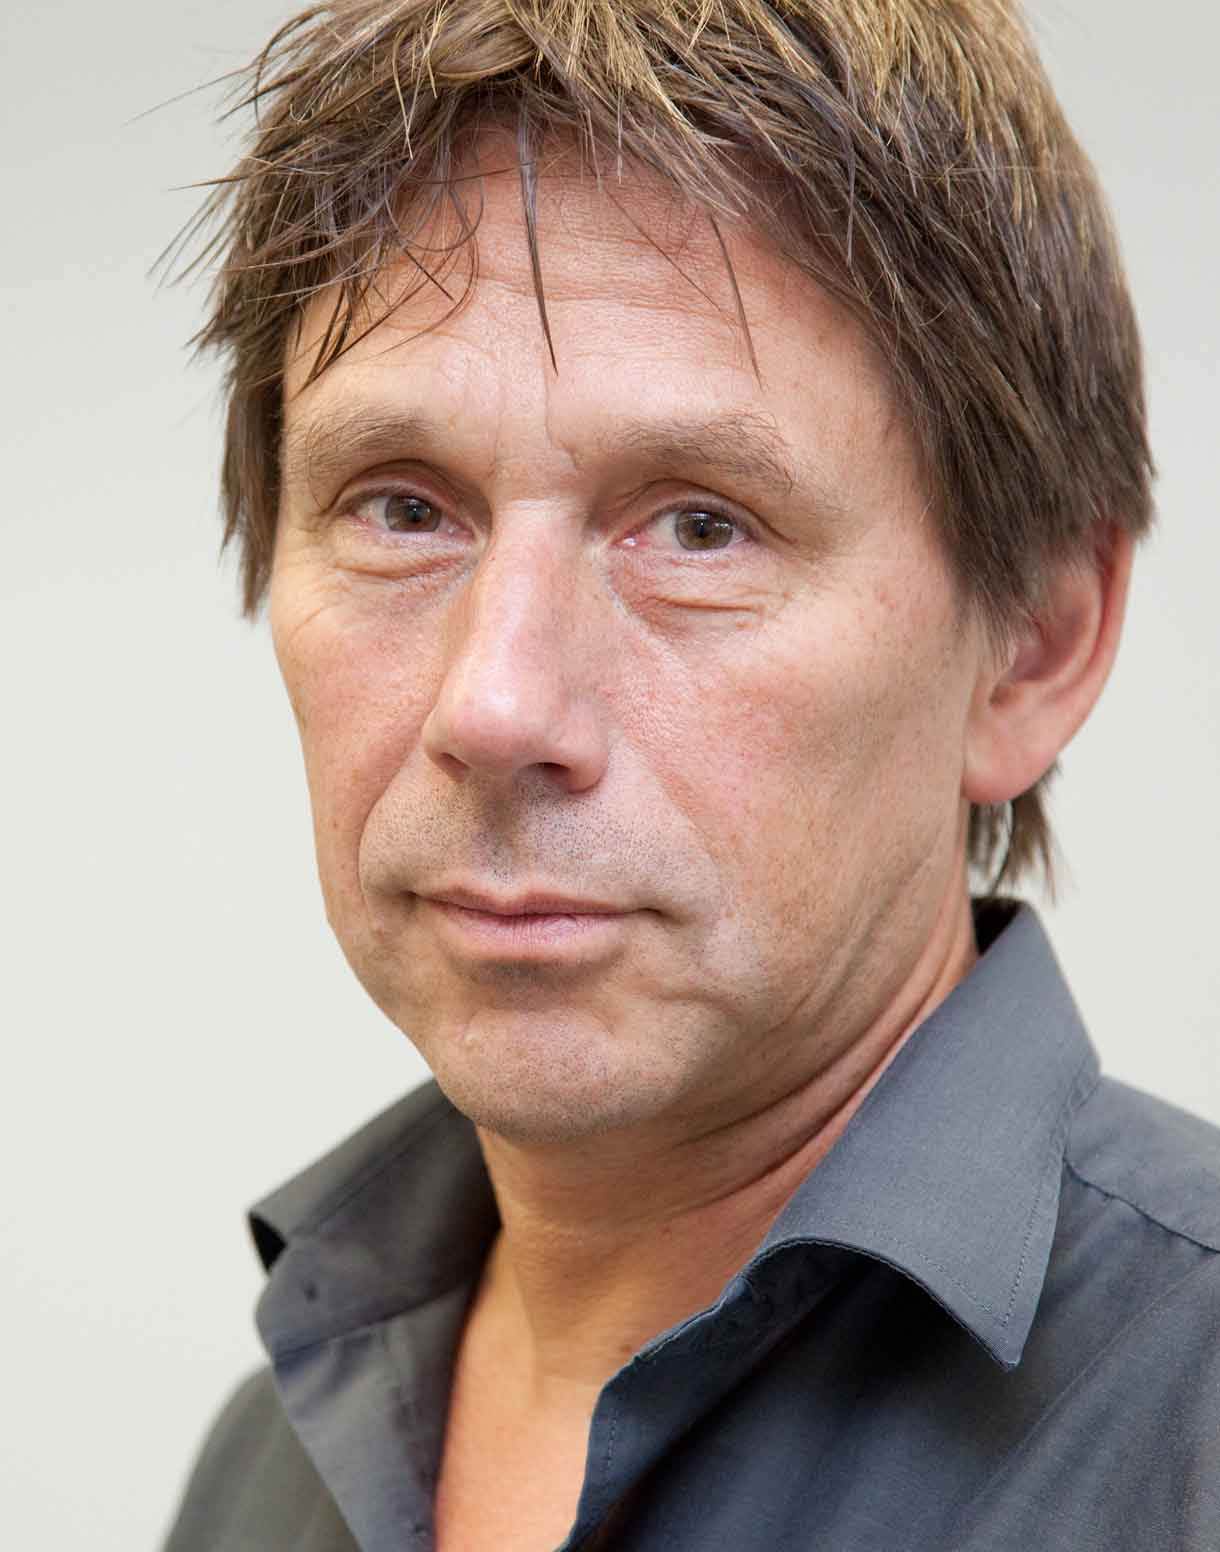
\includegraphics[width=1in,height=1.25in,clip,keepaspectratio]{img/Dillenbourg.jpg}}]{Pierre Dillenbourg}
% is ...
%\end{IEEEbiography}


\begin{IEEEbiography}[{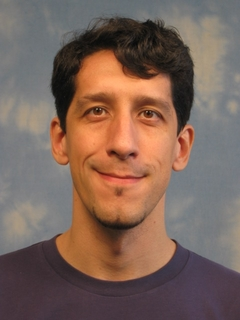
\includegraphics[width=1in,height=1.25in,clip,keepaspectratio]{img/LPPhoto.jpg}}]{Luis P. Prieto} received his Ph.D. in Information and Communication Technologies from the University of Valladolid (Spain). He is a Marie Curie Fellow at the CHILI Lab in the \'Ecole Polytechnique F\'ed\'erale de Lausanne (EPFL). His research interests include classroom orchestration, distributed and augmented paper learning technologies, and the use of wearable technologies to capture and understand complex practice with ICT and the use of such data for reflection. He has authored more than fifty academic publications on these topics, and he is a member of IEEE and ACM.
\end{IEEEbiography}


\begin{IEEEbiography}[{
\includegraphics[width=1in,height=1.25in,clip]{img/Sharma.png}}]{Kshitij Sharma}
 is ...
\end{IEEEbiography}

\begin{IEEEbiography}[{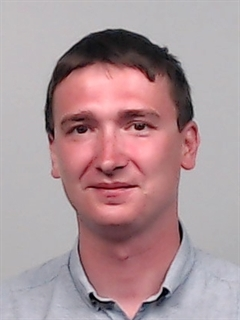
\includegraphics[width=1in,height=1.25in,clip,keepaspectratio]{img/Kidzinski.jpg}}]{{\L}ukasz~Kidzinski}
 is ...
\end{IEEEbiography}


\begin{IEEEbiography}[{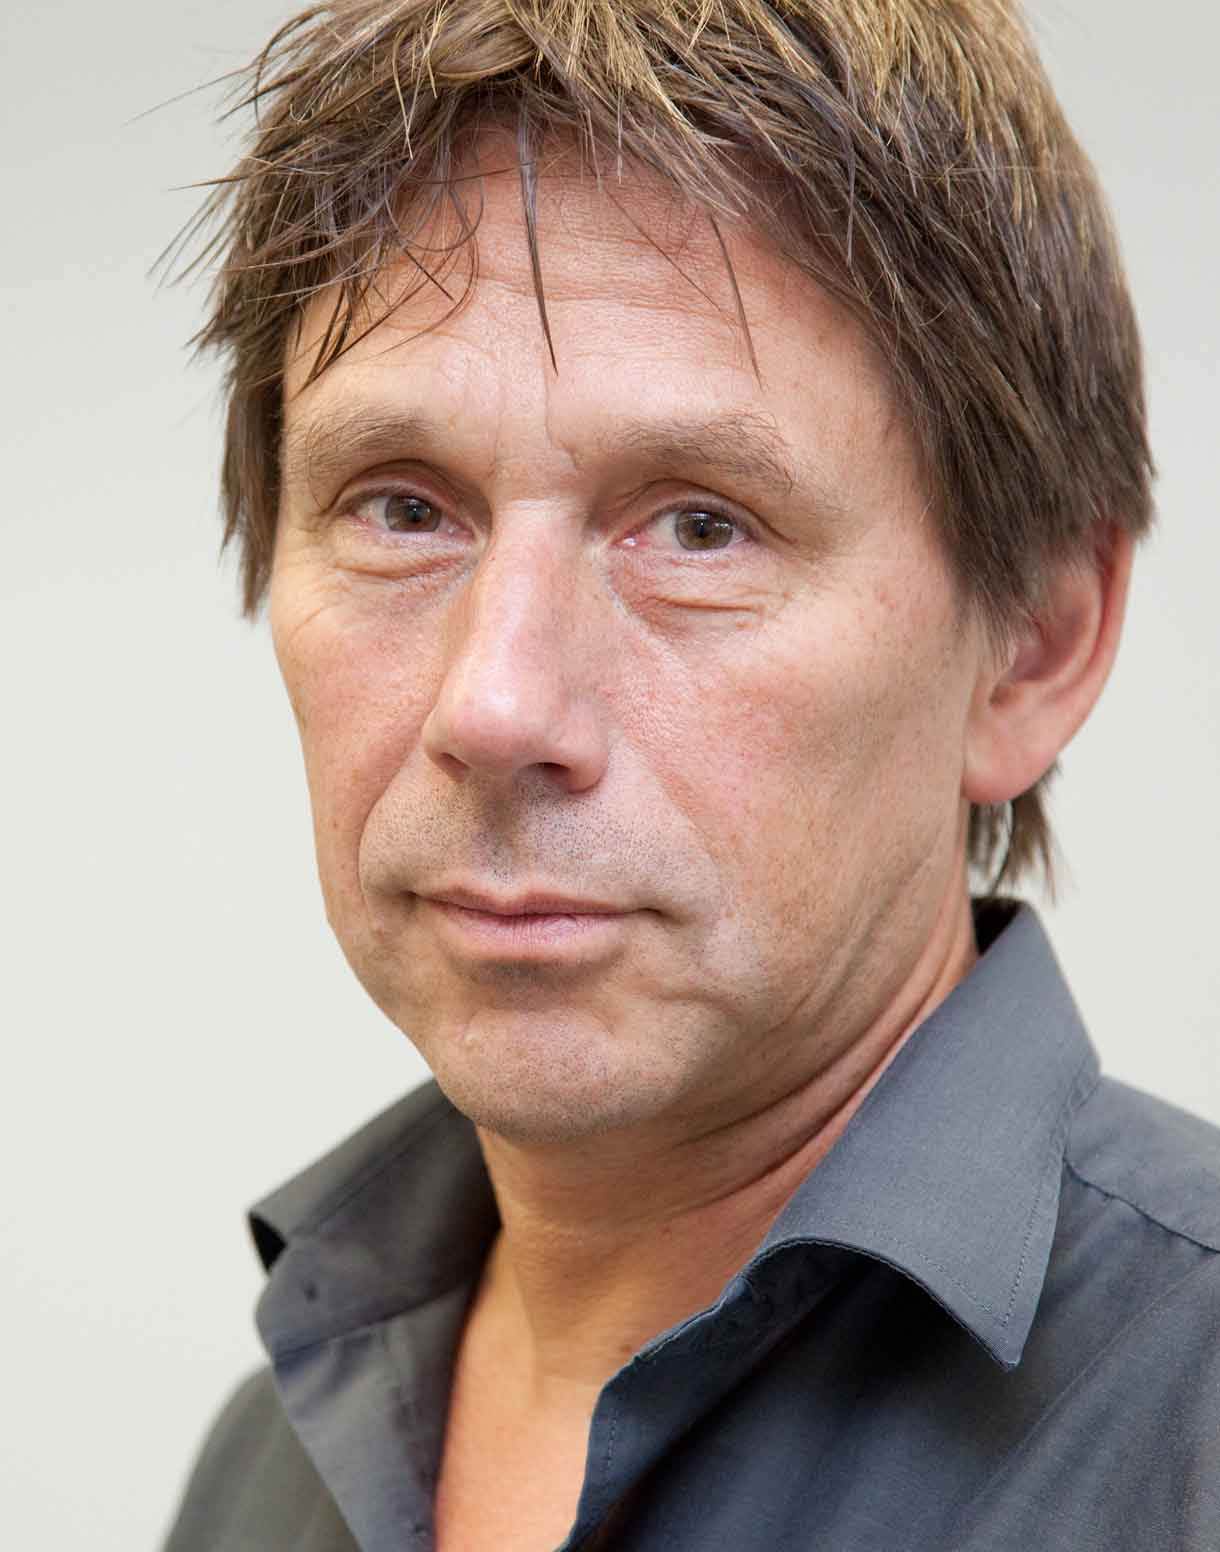
\includegraphics[width=1in,height=1.25in,clip,keepaspectratio]{img/Dillenbourg.jpg}}]{Pierre Dillenbourg} is a former school teacher and graduated in educational science (University of Mons, Belgium). He then obtained a PhD in computer science from the University of Lancaster (UK), in the domain of AI for educational software. After being assistant professor at the University of Geneva, he joined EPFL in 2002. He is currently full professor in learning technologies in the School of Computer \& Communication Sciences, where he is the head of the Computer-Human Interaction for Learning \& Instruction Lab. He is also the academic director at the Center for Digital Education, which implements the MOOC strategy of EPFL.
\end{IEEEbiography}

% You can push biographies down or up by placing
% a \vfill before or after them. The appropriate
% use of \vfill depends on what kind of text is
% on the last page and whether or not the columns
% are being equalized.

%\vfill

% Can be used to pull up biographies so that the bottom of the last one
% is flush with the other column.
%\enlargethispage{-5in}



% that's all folks
\end{document}


